\chapter{Ponderado de normales}
\label{chap:ponderadoNormales}
Se desea encontrar una forma de asignar las normales a la superficie que se usarán para hacer la iluminación. La manera propuesta sera crear primero una superficie implícita que envuelva la aproximación poligonal $\mathcal{A}_{\tau}$. La superficie implícita esta formada por funciones base, por lo tanto cada una de estas contribuye a la superficie y contribuye también a la forma como se van a modificar las normales. En este sentido en este trabajo entenderemos como \emph{ponderación} al proceso de ir sumando vectores que modifican la dirección de un vector normal. Dado que para hacer cálculos de iluminación los vectores deben ser unitarios, después de la ponderación hacemos un postproceso que nos asegure solo usar vectores unitarios. Por esta razón se hace énfasis en que las funciones base cambian \emph{la dirección} del vector normal.

\section{Representación implícita de superficies}
\label{sec:repImplicita}
Tradicionalmente en las GC hay dos formas de modelar superficies en el espacio $\mathbb{R}^3$ \cite{Blinn:metaballs}. Una de ellas es tener la superficie definida de manera paramétrica $s(\mu,\nu)$. Por lo tanto es posible crear una aproximación por medio de polígonos calculando los vértices mediante incrementos constantes en los parámetros.

Otra forma, es la llamada representación implícita. Que consiste en encontrar las soluciones de la siguiente ecuación:
\begin{equation}
 f(\textbf{x}) = 0,
\label{ec:supImplicita}
\end{equation}
donde $\textbf{x} \in \mathbb{R}^3$. Aunque ya se habían estudiado las superficies producidas por funciones de segundo grado, Blinn propuso una manera de generalizar estas superficies en \cite{Blinn:metaballs}. La idea de Blinn tenía el objetivo de representar estructuras moleculares donde los átomos se combinan con otros con transiciones graduales. Esta representación ha sido adoptada para realizar modelado de objetos orgánicos y funciones topológicamente muy complicadas. En el trabajo original una molécula es representada aproximadamente por medio de la combinación lineal de funciones suaves. En dicha representación, cada $j$-esimo átomo de la molécula es representado por una función suave $b_j$ ponderada por un coeficiente $c_j$ y centrada en el punto $\textbf{p}_j$ de la siguiente forma
\begin{equation}
 g(\textbf{x}) \approx \sum \limits_{j = 1}^{j} c_j b_j(\textbf{x} - \textbf{p}_j).
\label{ec:modeloBlobby}
\end{equation}

Blinn propuso utilizar la siguiente función $b$ (radialmente simétrica):
%. Se trata en representar cada átomo de una molécula como una función de densidad $b$ que en el centro del átomo $c_i$ es muy densa y decae suavemente mientras se aleja del centro una cierta distancia $r$. Por ejemplo la función:
\begin{equation}
 b(\alpha ; r) = e^{-\alpha r},
\label{ec:blobBlinn}
\end{equation}
donde $r$ es la distancia de $\textbf{x}$ al punto $\textbf{p}_i$ donde está centrada la función y $\alpha$ representa un parámetro de forma de la función (el ancho) .

Para llevar a cabo la visualización de \eqref{ec:modeloBlobby}, se define un umbral o isovalor $t$, por lo que se obtiene una superficie $S_t$ ver \eqref{ec:isosupeficie}, que se aproxima por poligonalización o por \emph{raycasting}. Claramente el resultado de la aproximación \eqref{ec:modeloBlobby} depende de la elección de los conjuntos $\{\textbf{p}_j\}$ y $\{c_j\}$ y de la elección de los parámetros de \eqref{ec:blobBlinn}, ver Figura \ref{fig:metaballs}.

\begin{figure}[htp]
  \begin{center}
    \subfigure[$\alpha$ pequeño]{\label{fig:metaball1}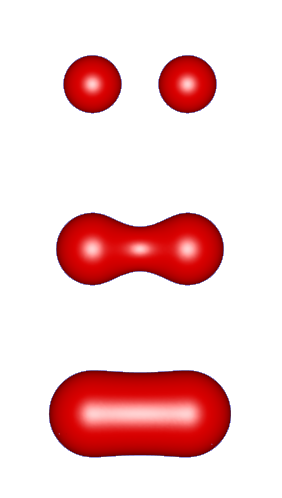
\includegraphics[scale=0.5]{img/cap02/blob01}}
    \subfigure[$\alpha$ mediano]{\label{fig:metaball2}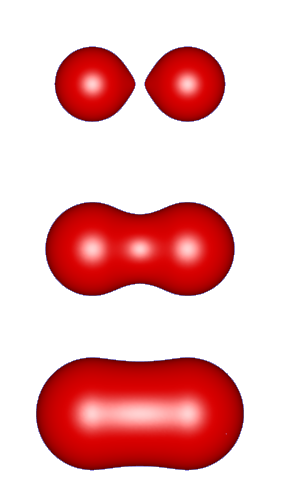
\includegraphics[scale=0.5]{img/cap02/blob02}}
    %\subfigure[$\alpha$ mediano]{\label{fig:metaball3}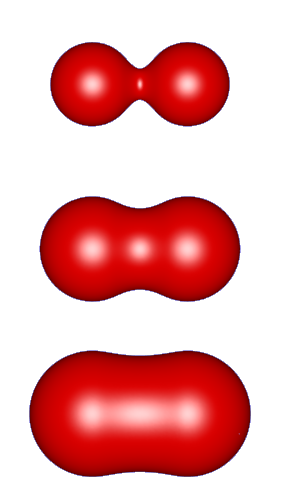
\includegraphics[scale=0.41]{img/cap02/blob03}}
    \subfigure[$\alpha$ grande]{\label{fig:metaball4}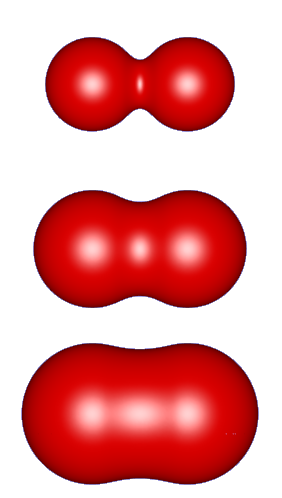
\includegraphics[scale=0.5]{img/cap02/blob04}}
  \end{center}
  \caption[Ilustración del efecto de \emph{blobbiness} para diferentes radios $r$ y $\alpha$ de blobs de Blinn]{Ilustración del efecto de \emph{blobbiness} para diferentes radios $r$ y $\alpha$ de blobs de Blinn. El umbral $t$ y la posición de los blobs se mantiene constante. El radio $r$ se incrementa de arriba a abajo y la $\alpha$ de izquierda a derecha.}
  \label{fig:metaballs}
\end{figure}

En la literatura de GC se conoce a la combinación lineal \eqref{ec:modeloBlobby} como \emph{modelo blobby} u orgánico y a las diversas funciones base $b$ como \emph{metaballs} o blobs. En \cite{NishimuraMetabolas} se propone la función base
\begin{equation}
\label{ec:metaballNishimura}
 b(\kappa, a; r) = \begin{cases}
            \kappa \left( 1 - \frac{3 r^2}{a^2} \right), & \text{si $0 \leq r \leq \frac{a}{3}$,} \\
	    \frac{3 \kappa}{2} \left( 1 - \frac{r}{a} \right)^2, & \text{si $\frac{a}{3} \leq r \leq a$,} \\
                    0, & \text{en otro caso,} \\
            \end{cases}
\end{equation}
donde $a$ representa la extensión o soporte de la función y $\kappa$ determina la densidad máxima de la función. En \cite{NishimuraMetabolas} los autores se refieren a \eqref{ec:metaballNishimura} como \emph{metaball}, dando origen al termino genérico \emph{metaballs}. En \cite{softObjects} se usa una función alternativa conocida como \emph{soft object}, definida como:
\begin{equation}
\label{ec:softObjects}
 b(\kappa, a; r) = \begin{cases}
            \kappa \left( 1 - \frac{4 r^6}{9 a^6} + \frac{17 r^4}{9 b^4} - \frac{22 r^2}{9 a^2}\right), & \text{si $0 \leq r \leq a$,} \\
	    0, & \text{en otro caso,} \\
            \end{cases}
\end{equation}
donde los parámetros $a$ y $\kappa$ representan los mismos conceptos que en \eqref{ec:metaballNishimura}.
%entonces encontrar y visualizar la superficie $S_{t}(\textbf{x}) = D(\textbf{x}) - t$. Después de hacer sustituciones algebraicas en la ecuación \eqref{ec:blobBlinn}, ésta puede ponerse en términos de dos parámetros $a_i(b_i, t, \alpha_i)$ que representa el radio de influencia de la función y de un parámetro de suavidad (\emph{blobbiness}) $\alpha_i(b_i, t)$.

%Aunque en \cite{Blinn:metaballs} se usa la función \eqref{ec:blobBlinn}, también queda claro que hay varias funciones $b$ que pueden ser usadas en su lugar. En gráficas por computadora todas las posibles funciones $b$ para usarse con este modelo se conocen como \emph{metaballs}, y en el campo de reconstrucción toman el nombre de \emph{blobs}. A la forma de representar una superficie\begin{equation}
 %v(\textbf{x}) \approx \sum \limits_{j = 1}^{J} c_j b_j (\textbf{x}) 
%\label{ec:modBlobby}
%\end{equation}se le conoce como \emph{modelo blobby}. La ecuación \eqref{ec:modBlobby} es una generalización de la ecuación \eqref{ec:blinnBlobby} para cualquier función base $b$. Las funciones base comúnmente dependen al menos de los parámetros $a$ y $\alpha$, que controlan el soporte y la suavidad respectivamente. 

%En la figura \ref{fig:metaballs}, se ilustran como dos blobs, con centro fijo, puestos uno a lado del otro, interactúan para formar una superficie implícita. Cuando dos o mas blobs se colocan de manera que sus soportes se intersequen empiezan a interactuar y pueden aproximar una superficie. A medida de que el soporte de la función $a$ y el parámetro de suavidad $\alpha$ de los blobs aumentan estos parecen unirse formando una superficie mas suave.
En la Figura \ref{fig:comBlobs} se muestra una comparación entre varias funciones blobs. El blob de \eqref{ec:blobBlinn} etiquetado como \emph{Blinn Gaussian}, el blob de \eqref{ec:metaballNishimura} etiquetado como \emph{Metaball}, el blob de \eqref{ec:softObjects} etiquetado como \emph{Soft Object} y el blob \emph{Kaiser-Bessel} que se analiza a detalle en la siguiente sección.

\begin{figure}[htp]
 \centering
  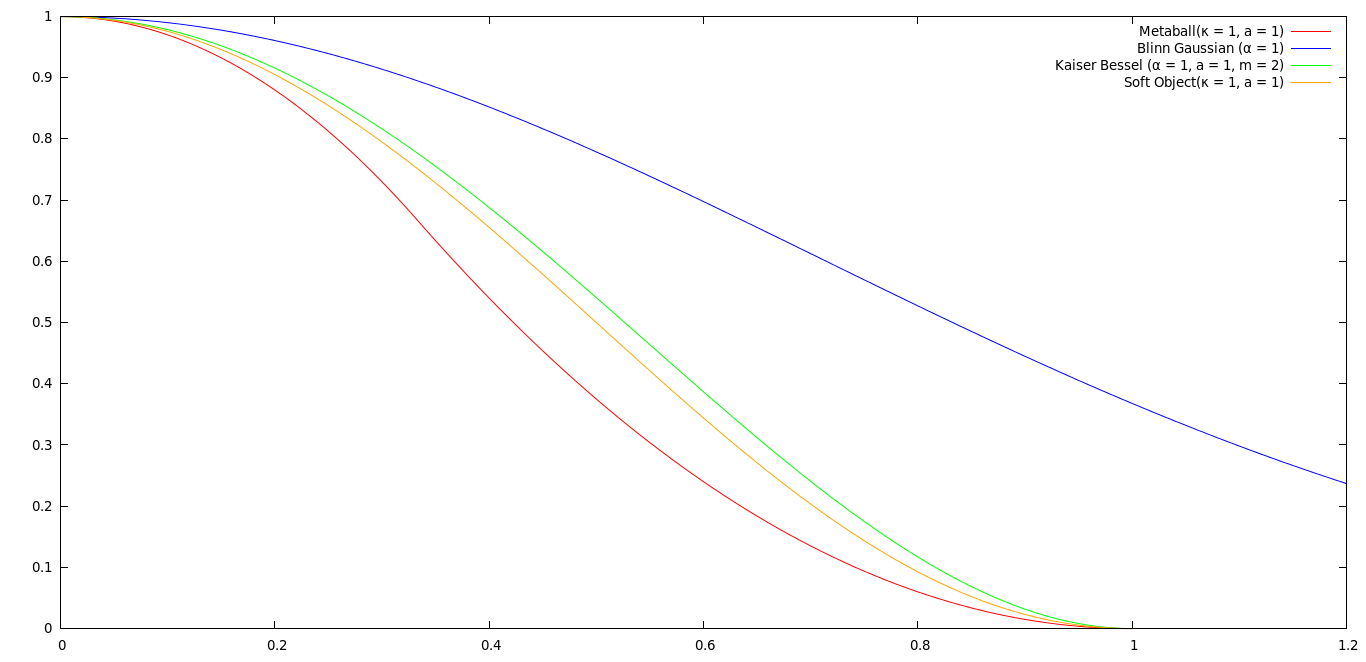
\includegraphics[scale=0.3]{img/cap02/comparision}
  \caption[Comparación entre las diferentes funciones blobs]{Comparación entre los diferentes blobs.}
  \label{fig:comBlobs}
\end{figure}

%Los blobs, han sido usados para fines de modelado orgánico en las GC \cite{BloomenthalTesis}. Varios blobs se han estudiado tanto para fines de reconstrucción \cite{LewitAlternatives}y \cite{LewitPractical} como de visualización \cite{NishimuraMetabolas} y \cite{MurakiBlobby}.

%Para poder visualizar una superficie implícita de la forma \eqref{ec:modBlobby} con iluminación, es necesario conocer el gradiente $\nabla b$, de las funciones base. Como la superficie es una combinación lineal de las funciones base podemos aproximar el gradiente de la superficie como una combinación lineal de los gradientes de los blobs. El gradiente es un vector normal $\vec{n}$ a la superficie \cite{bussCG} que como se dijo en el capítulo anterior es necesario para hace los cálculos de iluminación.

\subsection{Las funciones Kaiser-Bessel generalizadas (\textit{blobs})}

La aproximación \eqref{ec:modeloBlobby} también sirve para modelar funciones de densidad en el área de reconstrucción a partir de proyecciones (un problema inverso cuyo ejemplo mas típico son los instrumentos médicos que realizan tomografías \cite{tomografyBook}). En particular son usados en aquellos métodos basados en expansiones en series de funciones base. En este campo también se han usado varias funciones base tales como vóxeles. Pero una función base que ha resultado en buenas aproximaciones son las funciones Kaiser-Bessel generalizadas \cite{BlobsMate}, definidas como:
%Las funciones Kaiser Bessel eran conocidas en el procesamiento de imágenes, pero fueron generalizadas por Lewitt en \cite{BlobsMate}. Ahí describe matemáticamente las funciones que nosotros llamaremos \emph{blobs} (De aquí en adelante al decir \emph{blob} me referiré a este blob). Los blobs han mostrado ser funciones bases ideales para aproximar volúmenes para propósitos de reconstrucción. Ver por ejemplo \cite{LewitAlternatives}, \cite{LewitPractical} y \cite{EdgarOptimization}.
%Los blobs que Lewitt describe son:
\begin{equation}
\label{ec:blob}
 b(m, \alpha, a; r) = \begin{cases}
            \dfrac{ I_m \left(  \alpha \sqrt{1 - \left( \frac{r}{a} \right) ^2 }  \right) } {I_m(\alpha)} \left( \sqrt{1 - \left( \frac{r}{a} \right) ^2 }  \right)^m, & \text{si $0 \leq r \leq a$,} \\
                    0, & \text{en otro caso,} \\
            \end{cases}
\end{equation}
en donde $r$ es la distancia radial al centro del blob, $I_m$ es la función Bessel modificada de orden $m$, $a$ determina el soporte y $\alpha$ es el parámetro que controla la forma de la función. 

La elección de las funciones Kaiser-Bessel generalizadas se debe a sus propiedades adecuadas para el área de procesamiento de imágenes, tales como la continuidad en el soporte finito y su rápida tasa de desvanecimiento en su espectro (algo que se considera como ancho de banda limitado en la practica), ver Figura \ref{fig:blobSpectre}. De hecho, estas funciones son muy conocidas en al área de procesamiento de señales donde son utilizadas típicamente como ventanas (\emph{windows} en ingles). De ahora en adelante al usar el termino \emph{blob} nos referiremos a la función base de \eqref{ec:blob}.

\begin{figure}[htp]
 \centering
  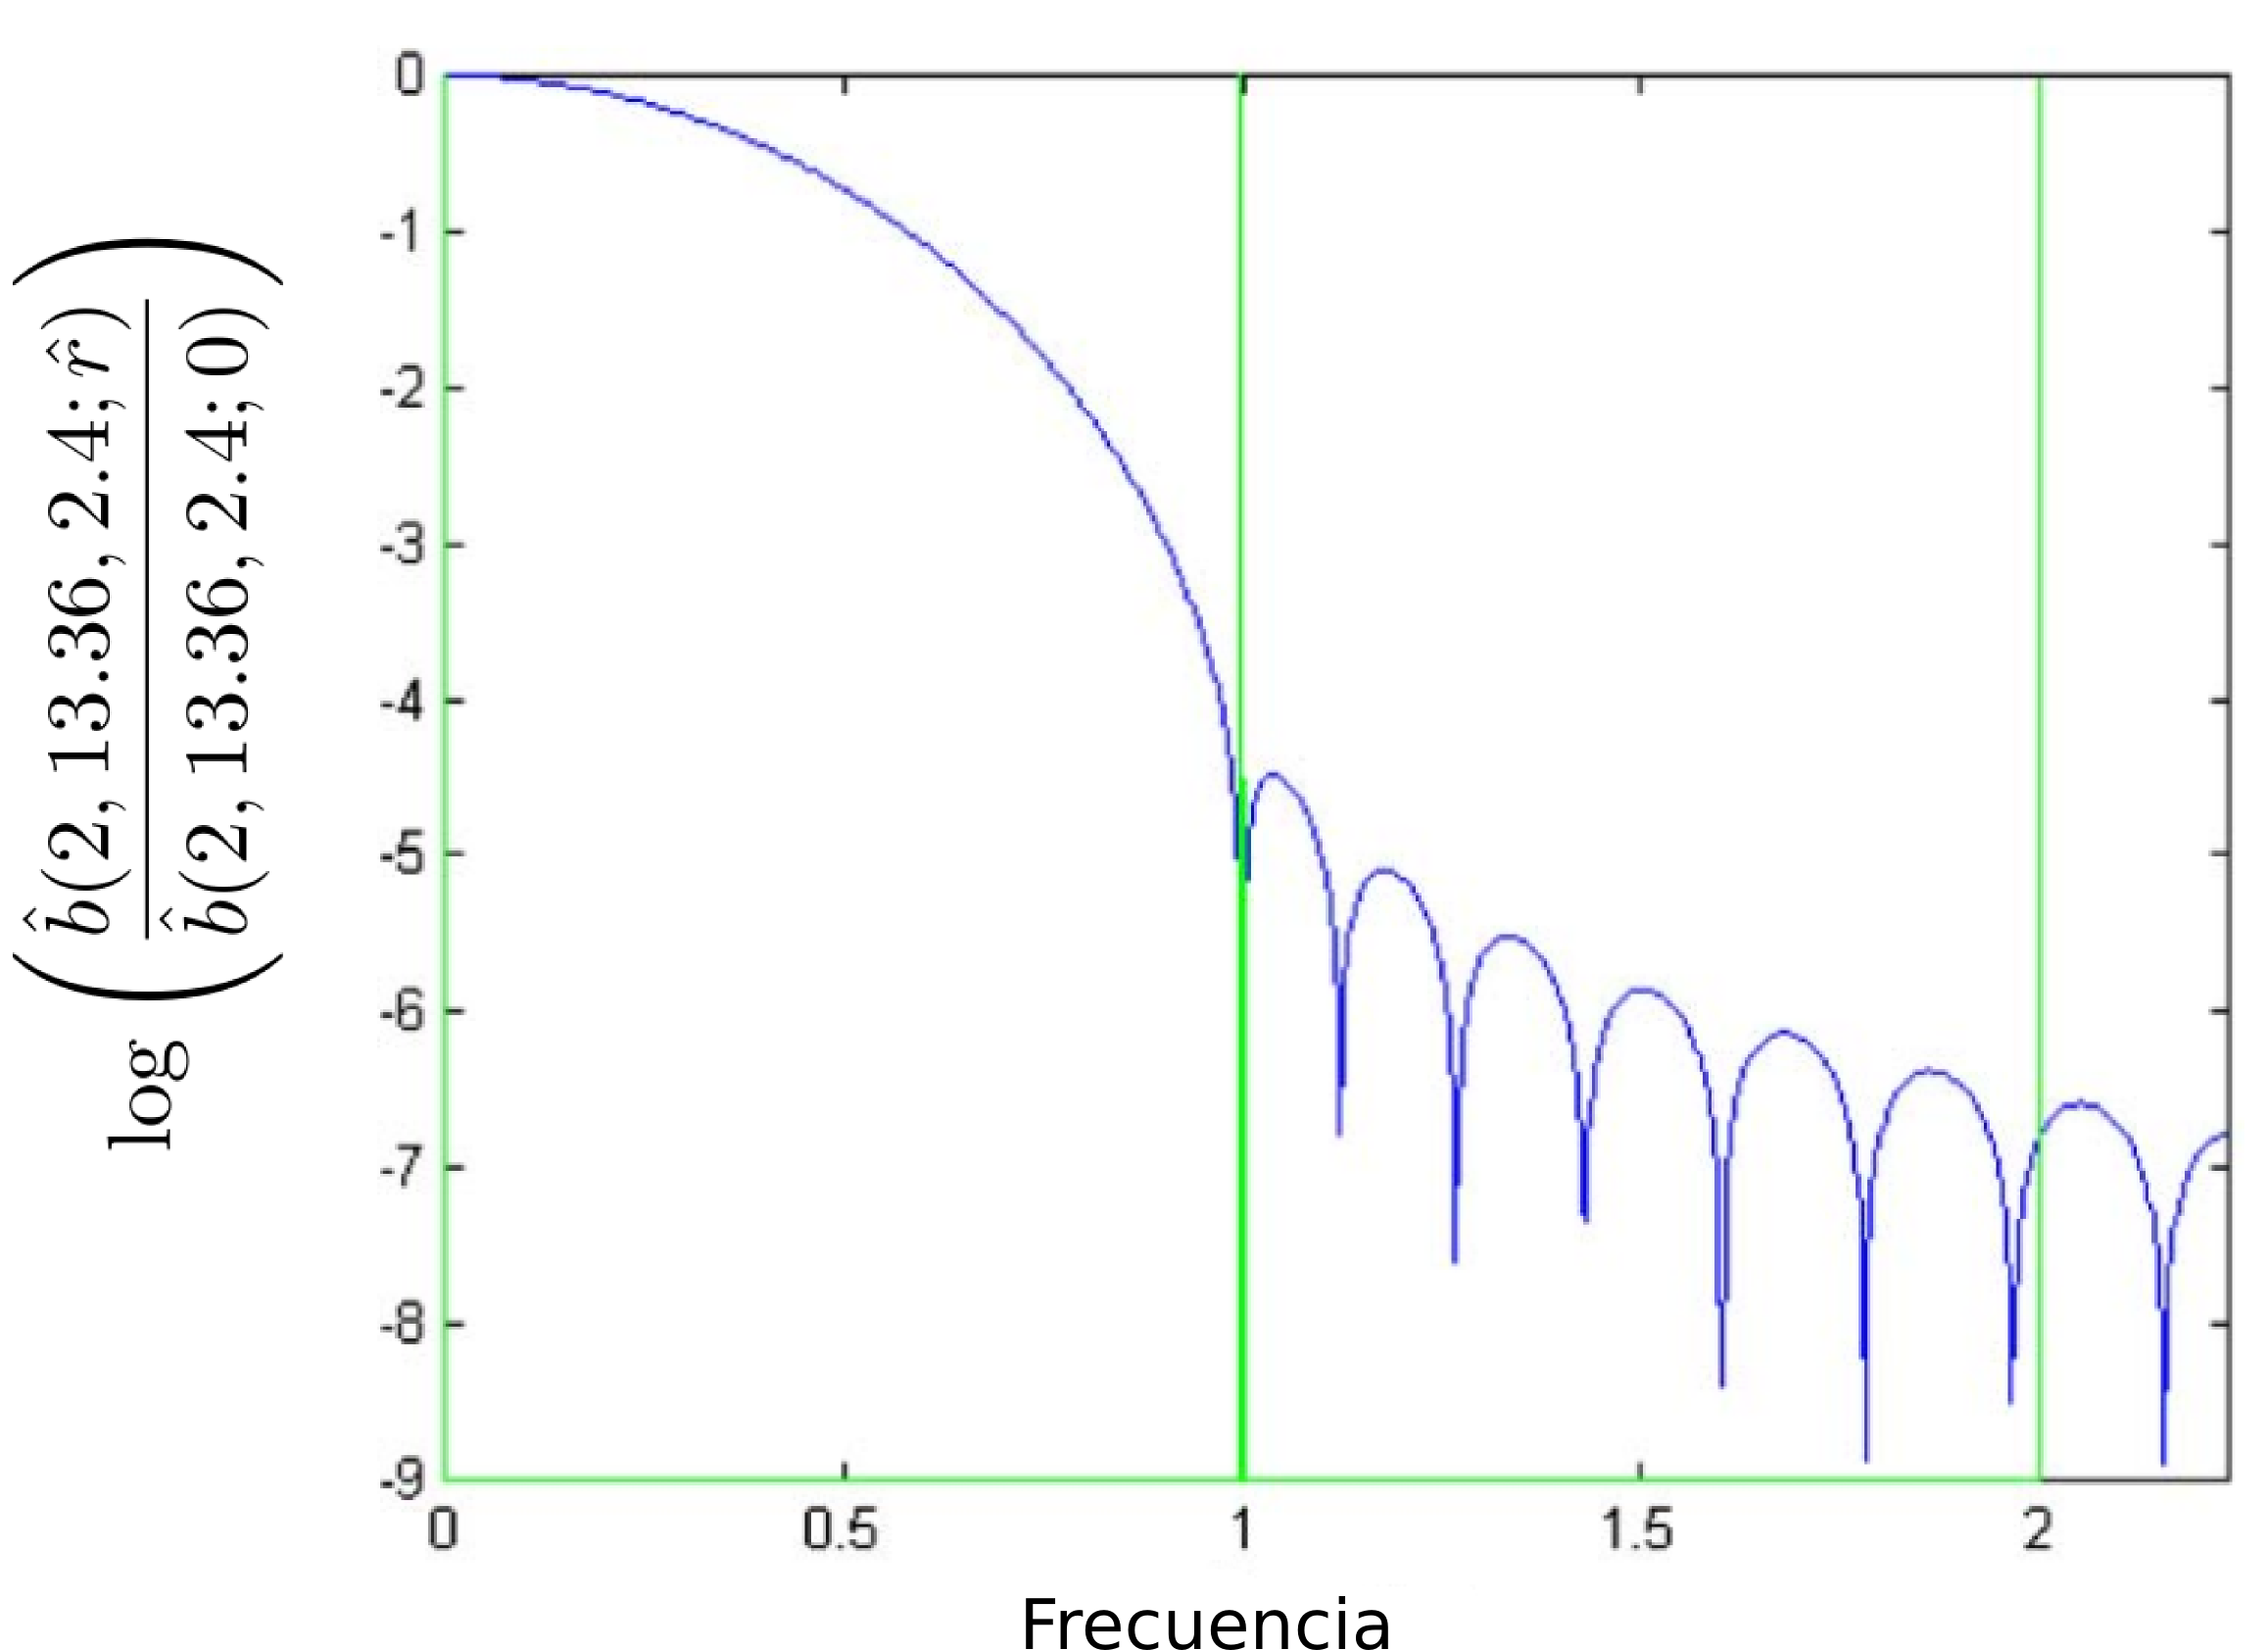
\includegraphics[scale=0.9]{img/cap02/blobSpectre}
  \caption[Espectro del blob en escala logarítmica]{Aquí se gráfica la magnitud de la transformada de Fourier del blob (espectro) en escala logarítmica contra la distancia radial $\hat{r}$ al centro del blob (frecuencia).}
  \label{fig:blobSpectre}
\end{figure}

%Debido a que el blob es una función radialmente simétrica, podemos obtener información valiosa de los perfiles del mismo. Es decir construyendo una gráfica de su valor variando su radio. Por ejemplo la variación del parámetro $a$ nos dice a partir de que valor el blob deja de tener influencia en la densidad (toma valor de cero) esto se puede ver en la figura \ref{fig:blobRadiusVariation}.

% \begin{figure}[htp]
%  \centering
%   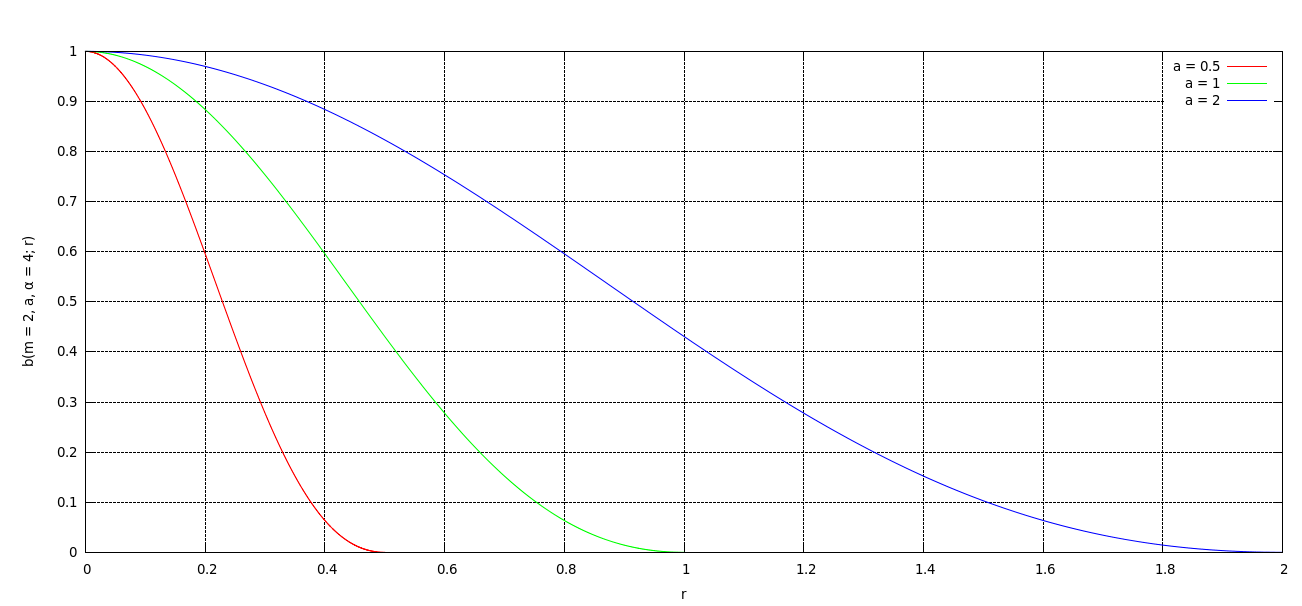
\includegraphics[scale=0.35]{img/cap02/BlobRadiusM2AL4}
%   \caption[Comparación entre blobs de diferente soporte]{La gráfica muestra el valor del blob $b$, conforme varía la distancia al centro $r$. Se fijan los parámetros $m = 2$ y $\alpha = 4$, y se grafican blobs de diferente soporte $a$.}
%   \label{fig:blobRadiusVariation}
% \end{figure}

El orden $m$ del blob es un entero positivo que determina el número de derivadas que tiene la función en su punto $a$. Como es bien sabido este parámetro está relacionado con la tasa de cambio de la función y en visualización es comúnmente asociado con la suavidad de la función. Para el orden dos, el blob es ya una función suave que tiene derivada en todo el soporte, además nadie ha demostrado que elecciones de $m$ mayores sean mas efectivas. Por lo que al igual que en \cite{EdgarOptimization}, aquí fijaremos el valor $m = 2$. 

Otro parámetro que afecta la forma del blob es el parámetro $\alpha$, mientras $\alpha$ sea más pequeño el blob decae más lentamente. La Figura \ref{fig:blobSmothness} muestra la variación del blob con respecto a $\alpha$, dejando como constantes $a = 1$ y $m = 2$.

% \begin{figure}[htp]
%   \begin{center}
%     \subfigure[$m = 0$]{\label{fig:blobM0}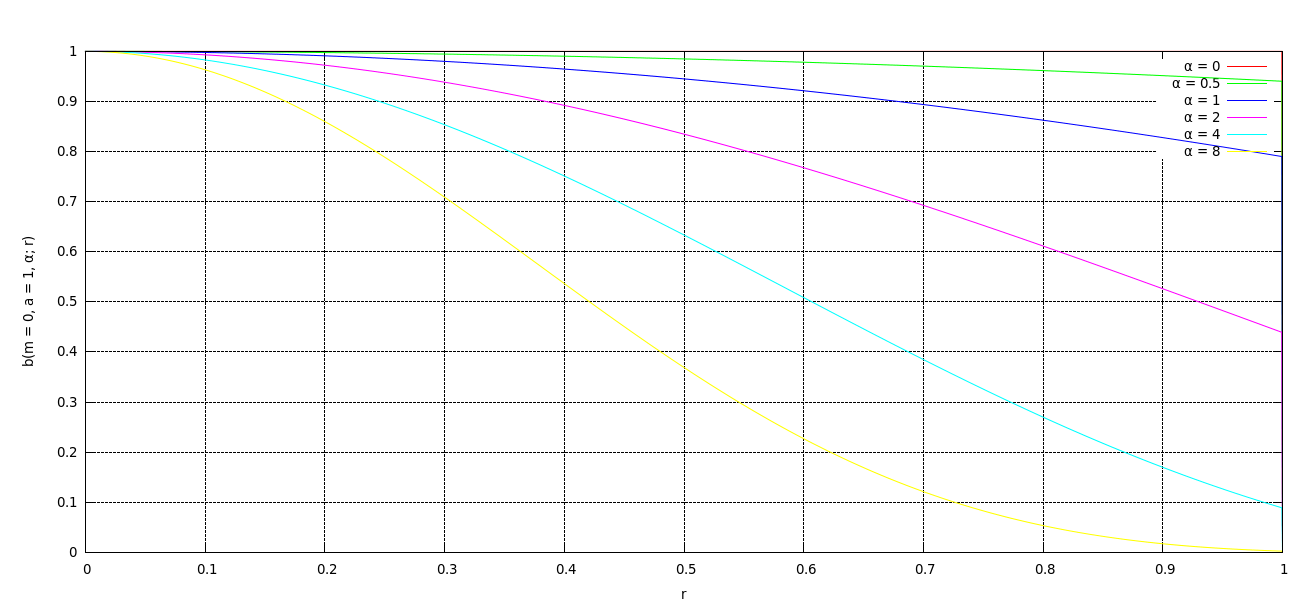
\includegraphics[scale=0.3]{img/cap02/GraficaM0A1}} \\
%     \subfigure[$m = 1$]{\label{fig:blobM1}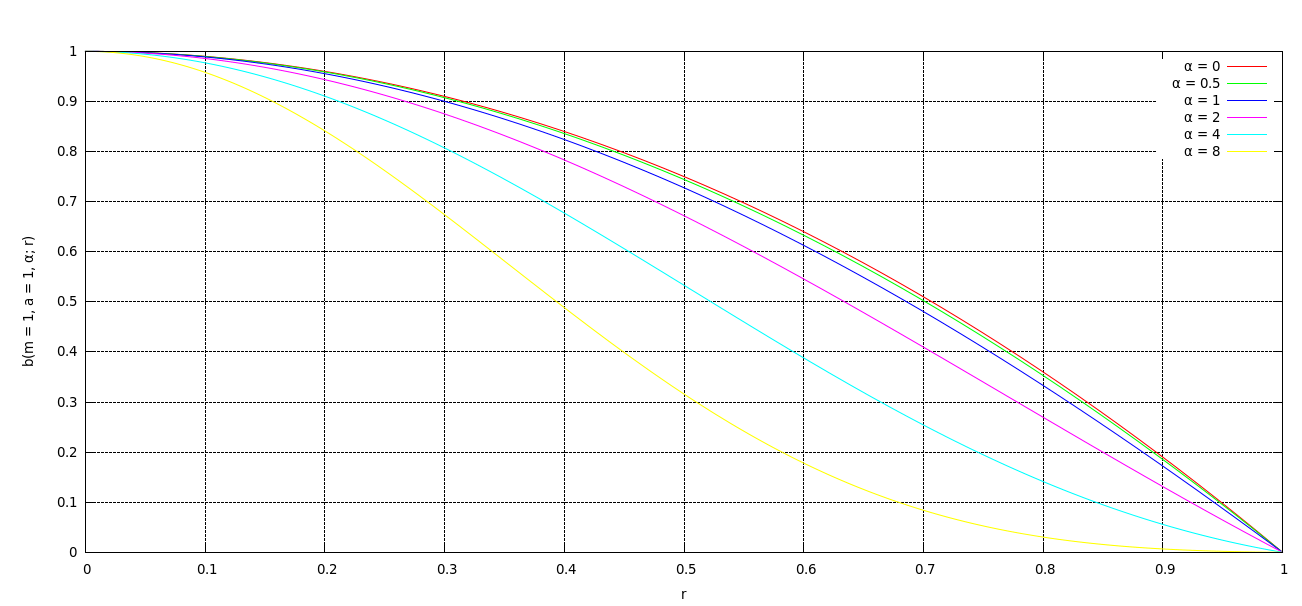
\includegraphics[scale=0.3]{img/cap02/GraficaM1A1}} \\
%     \subfigure[$m = 2$]{\label{fig:blobM2}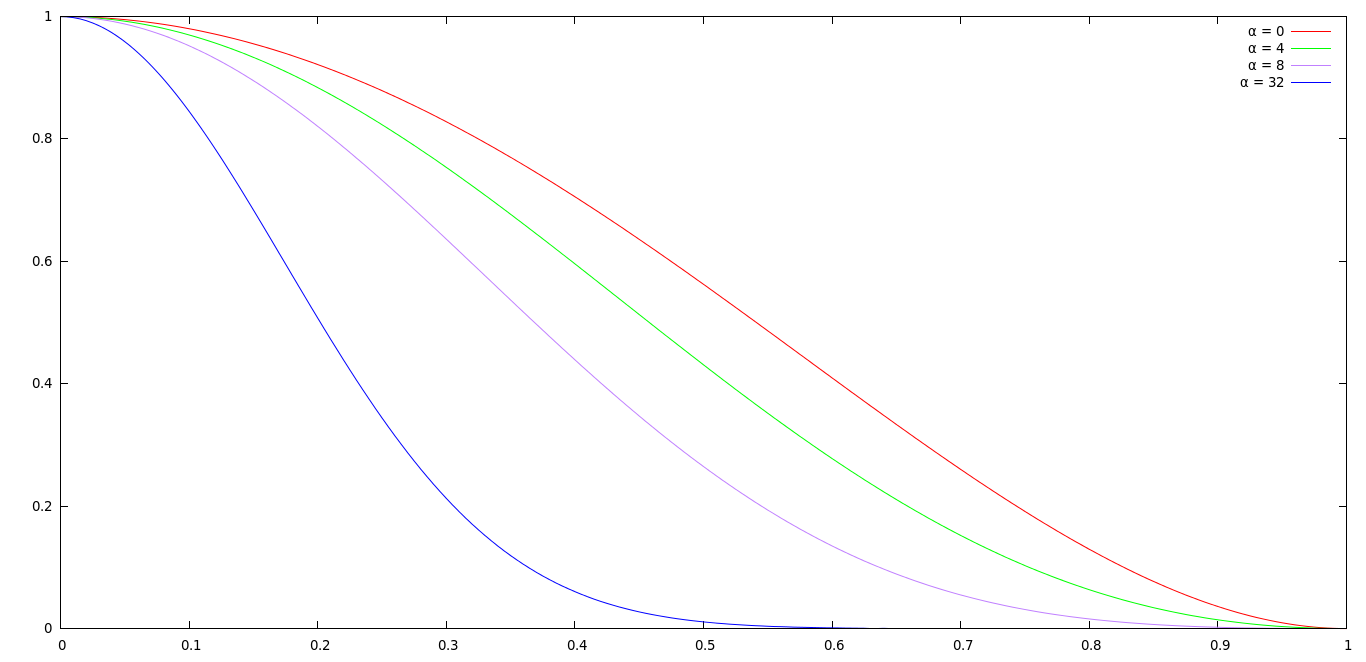
\includegraphics[scale=0.3]{img/cap02/GraficaM2A1}} \\
%   \end{center}
%   \caption[Variación de los parámetros de suavidad del blob]{En esta figura se muestra como afecta al blob que se cambien el orden $m$ y el parámetro de suavidad $\alpha$, conforme éste ultimo aumente el blob parece decaer mas rápido.}
%   \label{fig:blobSmothnessVariation}
% \end{figure}


\begin{figure}[htp]
 \centering
  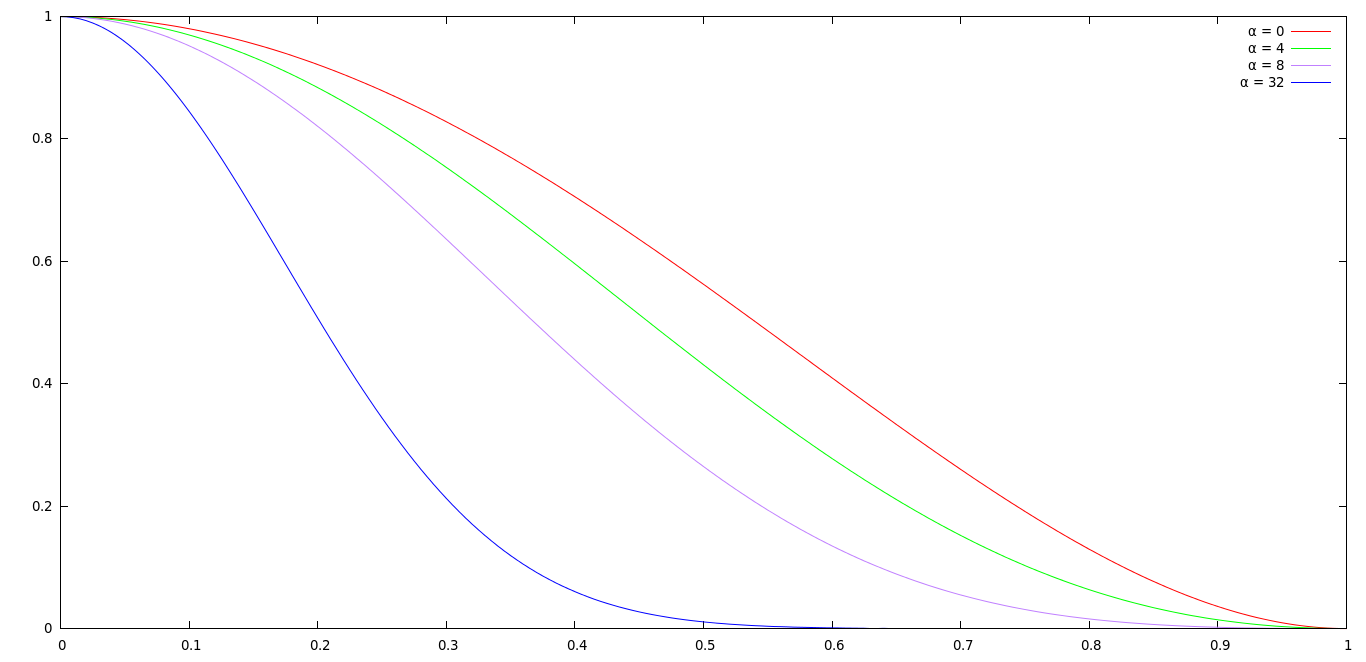
\includegraphics[scale=0.3]{img/cap02/GraficaM2A1}
  \caption[Ilustración de diferentes blobs con $a = 1$ y $m = 2$ variando $\alpha$]{Ilustración de diferentes blobs con $a = 1$ y $m = 2$ variando $\alpha$ en el blob de \eqref{ec:blob}, mientras $\alpha$ aumenta el blob decae mas rápido.}
  \label{fig:blobSmothness}
\end{figure}

En este trabajo utilizaremos la aproximación \eqref{ec:modeloBlobby}, con las funciones base definidas por \eqref{ec:blob} para poner normales sobre la malla $\mathcal{A}_{\tau}$ generada por el algoritmo de Artzy y visualizar usando el modelo de \eqref{ec:phongModelo}. Como hemos mencionado antes, para hacer iluminación es necesario conocer el gradiente a la superficie y consecuentemente la normal \cite{bussCG}.

Para la aproximación \eqref{ec:modeloBlobby} el gradiente se obtiene como
\begin{equation}
\nabla g (\textbf{x}) = \nabla \sum \limits_{j = 1}^{j} c_j b_j(\textbf{x} - \textbf{p}_j) = \sum \limits_{j = 1}^{j} c_i \nabla b_j(\textbf{x} - \textbf{p}_j).
 \label{ec:modBlobbyGradiente}
\end{equation}
Esto quiere decir que el gradiente de la superficie (y por ende un vector normal a la superficie) se puede obtener sumando las contribuciones de los gradientes de cada blob que forma la superficie.
%De la figura \ref{fig:blobSmothnessVariation} podemos ver que en general mientras $\alpha$ y $m$ aumenten el blob tiene una transición más suave. En el caso extremo cuando $\alpha = 0$ y $m = 0$, el blob se convierte en una función escalón que pasa de $1$ a $0$ justo al acabar el soporte. 
 
%\subsubsection{Gradiente y transformada de Fourier del blob}

%También se dan formulas para calcular la transformada de Fourier $\hat{b}$ del blob y el gradiente $\nabla b$. El gradiente del blob puede ser escrito como:
En \cite{BlobsMate} Lewitt ha proporcionado una forma analítica para obtener el gradiente de \eqref{ec:blob} como sigue:

\begin{equation}
  \frac{\partial b}{\partial r} = 
    \begin{cases} 
      \left[ \dfrac{-1 / \alpha }{\alpha^{m - 2} I_{m}(\alpha)} \right] (r / a) z^{m - 1} I_{m - 1}(z), & \text{si $0 \leq r \leq a$,} \\
      0, & \text{en otro caso,} \\                                
    \end{cases}
\label{ec:blobGradient}
\end{equation}
en donde $z = \sqrt{\alpha (1 - (r / a)^2)}$.

Para una función radialmente simétrica el gradiente puede calcularse fácilmente como
\begin{eqnarray}
 \nabla b(\textbf{x} - \textbf{p}_j) & = & \nabla b (r (\textbf{x} - \textbf{p}_j)) \\
 \nonumber
	  & = & \frac{\partial b}{\partial r} \frac{\partial}{\partial \textbf{x}} r (\textbf{x} - \textbf{p}_j),
\end{eqnarray}
donde $r$ es la función de distancia euclidiana $r(\textbf{x} - \textbf{p}_j) = \sqrt{ \sum \limits_{i = 1}^{3} (x_i - p_{i,j})^2}$. Es fácil ver que $\frac{\partial}{\partial \textbf{x}} r (\textbf{x} - \textbf{p}_j) = \frac{\textbf{x} - \textbf{p}_j}{|\textbf{x} - \textbf{p}_j|}$, por lo tanto podemos concluir que:
\begin{equation}
 \nabla g(\textbf{x}) = \sum \limits_{j = 1}^{j} c_j \frac{\partial b}{\partial r} \left( \frac{\textbf{x} - \textbf{p}_j}{|\textbf{x} - \textbf{p}_j|} \right).
 \label{ec:gradSuperficie}
\end{equation}
Esto quiere decir que el gradiente es un vector que va del centro $\textbf{p}_j$ del blob hasta el punto $\textbf{x}$ cuya magnitud es $\frac{\partial b}{\partial r}$. Finalmente, se muestra en la Figura \ref{fig:gradientValueComparision} la gráfica del blob $b(r)$ y de su gradiente $\frac{\partial b}{\partial r}$.

%En donde $\textbf{c}$ es el centro del blob. La normal a la superficie del blob puede verse como un vector cuya magnitud es el escalar $\frac{\partial b}{\partial r}$ y dirección $\textbf{p} = \textbf{x} - \textbf{c}$. Lewitt proporciona en \cite{BlobsMate} una forma de calcular la magnitud:

%En donde $z = \sqrt{\alpha [1 - (r / a)^2]}$. Por lo tanto podemos calcular la normal a cada punto de la superficie. Simplemente sumamos todos los gradientes de las funciones base que afecten al punto y luego normalizamos.

%La figura \ref{fig:blobGradientVariation} muestra como varía el gradiente del blob conforme cambia el parámetro $\alpha$, como puede apreciarse el gradiente siempre tiene valor negativo.

% \begin{figure}[htp]
%  \centering
%   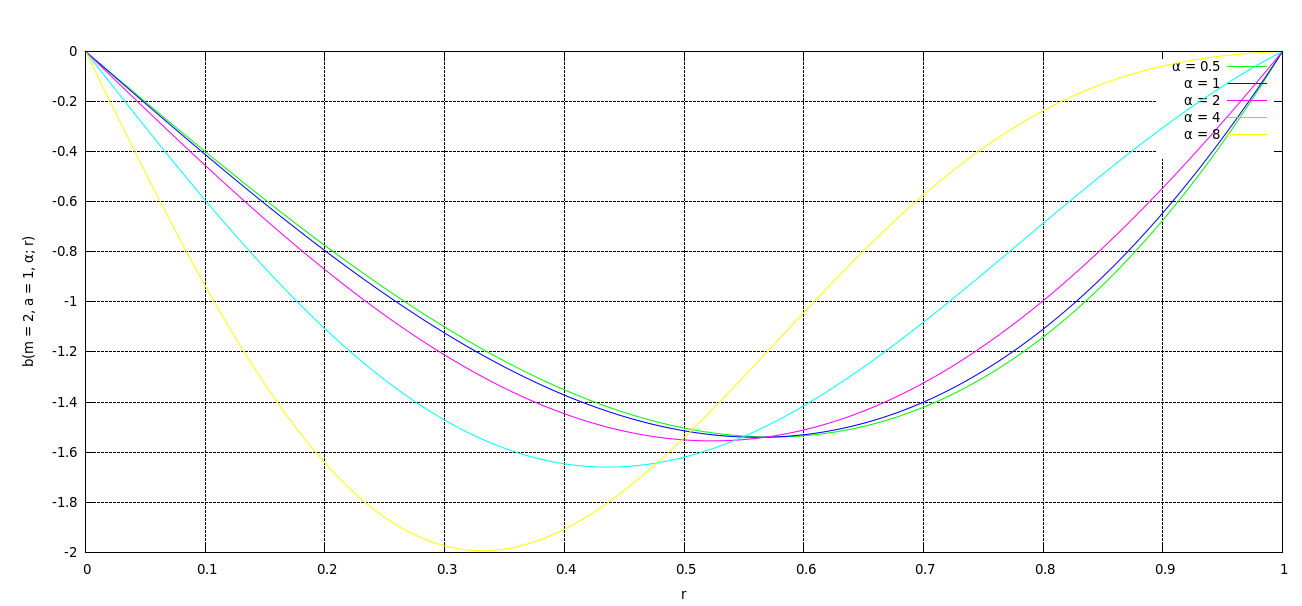
\includegraphics[scale=0.35]{img/cap02/BlobGradientM2A1}
%   \caption[Variación del gradiente del blob.]{La gráfica muestra el valor del blob $b$, conforme varía la distancia al centro $r$. Se fijan los parámetros $m = 2$ y $a = 1$.}
%   \label{fig:blobGradientVariation}
% \end{figure}


\begin{figure}[htp]
 \centering
  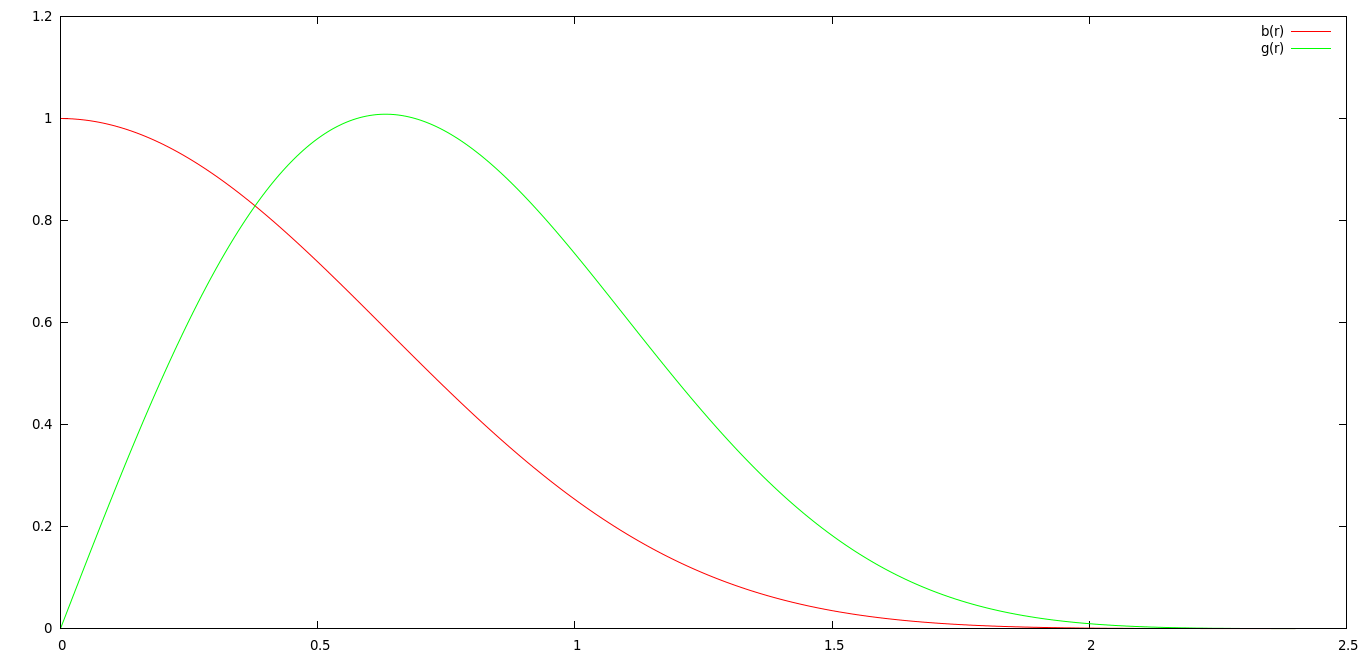
\includegraphics[scale=0.3]{img/cap02/BlobGradien}
  \caption[Comparación entre el blob y su gradiente]{La gráfica muestra el valor del blob con parámetros $b(a = 2.4, \alpha = 13.36, m = 2)$ y la magnitud de su gradiente calculado con \eqref{ec:blobGradient}.}
  \label{fig:gradientValueComparision}
\end{figure}


% La transformada de Fourier del blob, que nos servirá para hacer una optimización en la sección posterior también se calcula en \cite{BlobsMate} y se define de la siguiente manera cuando $m = 2$:
% 
% \begin{equation}
% \label{ec:blobFT}
%  \hat{b}(2, \alpha, a; R) = \dfrac{(2 \pi)^{3/2} a^3 \alpha^2}{I_2(\alpha)}\begin{cases}
%             \dfrac{ I_{ 7 / 2 } \left( \sqrt{ \alpha^{2} - (2 \pi a R)^{2}}  \right) } { \left( \sqrt{\alpha^2 - (2 \pi a R) ^2}  \right)^{ 7 / 2 }} & \text{si $2 \pi a R \leq \alpha$} \\
%             \dfrac{ J_{ 7 / 2 } \left( \sqrt{ (2 \pi a R)^{2} - \alpha^{2}}  \right) } { \left( \sqrt{(2 \pi a R)^{2} - \alpha^{2}}  \right)^{ 7 / 2 }} & \text{si $2 \pi a R \geq \alpha$} \\
%             \end{cases}
% \end{equation}
% 
% En donde $J_i$ es la función Bessel de orden $i$.
\section{Contribución de la tesis}
El objetivo de el trabajo es poder mejorar la calidad visual de la malla de Arzy $\mathcal{A}_{\tau}$ por medio de técnicas de GC. 

Para este fin se planea modificar los vectores normales a la superficie y usar el modelo de iluminaciónde Phong \ref{ec:phongModelo}. La manera como se hace esta modificación es creando una superficie implicita que envuelve la malla $\mathcal{A}_{\tau}$ y calculando las normales en dicha superficie implicita.

La primera aportación del trabajo consistio en encontrar los parametros de los blobs para visualización en tres configuraciones del conjunto $\{ \textbf{p}_j \}$. Aunque se usa el método descrito en \cite{EdgarOptimization} en dicho trabajo solo se obtienen parámetros para una configuración.

La aportación mas importante es la manera como se construye la malla con la que se hace la ponderación de las normales. Este proceso es descrito en la sección \ref{sec:ponderadoNormalesBlobs}.

Finalmente, también se hacen experimentos para probar la tecnica propuesta en la esta sección. Dichos experimentos son explicados en el capítulo \ref{chap:experimetos} y tambien constituyen una aportación.

\subsection{Optimización de blobs para visualización}
\label{sec:optiBlobs}
Claramente la elección de los parámetros $\alpha$, $a$, $m$ y la distribución de las funciones bases $\{ \textbf{p}_j \}$ afectará los resultados de la aproximación \eqref{ec:modeloBlobby}. Debido a que en GC se conoce con toda certeza la función a modelar es posible seleccionar un conjunto $\{ b_j \}$ con diferentes funciones base o una función base con diferentes parámetros correspondientes. Por ejemplo, en regiones muy homogéneas se pueden utilizar funciones mas anchas y en regiones con mas detalle usar funciones mas finas. En contraste, en el caso de la reconstrucción no se conoce, en general, la naturaleza de la función $v$ a aproximar, por lo tanto se usa una función base cuyos parámetros tienen que ser determinados bajo un criterio que tome en cuenta la distribución del conjunto $\{ \textbf{p}_j \}$. 

Existen varias posibles distribuciones del conjunto $ \{ \textbf{p}_j \} $, llamadas rejillas. En este trabajo nos interesan las tres siguientes:

\begin{enumerate}
\item La rejilla cubica simple (\emph{sc}) definida por
\begin{equation}
 G_\Delta = \{ \Delta \textbf{x} | \textbf{x} \in \mathbb{Z}^3 \}.
 \label{ec:rejillaSC}
\end{equation}

\item La rejilla \emph{bcc} que viene del termino \emph{body centered cubic grid}, que se define como
\begin{equation}
 B_\Delta = \{ \Delta \textbf{x} | \textbf{x} \in \mathbb{Z}^3 \text{ y con } x_1 \equiv x_2 \equiv x_3 \pmod 2 \}.
 \label{ec:rejillaBCC}
\end{equation}

\item La rejilla \emph{fcc} o \emph{face centered cubic grid} definida como
\begin{equation}
 F_\Delta = \{ \Delta \textbf{x} | \textbf{x} \in \mathbb{Z}^3 \text{ y con } x_1 + x_2 + x_3 \equiv 0  \pmod 2 \}.
 \label{ec:rejillaFCC}
\end{equation}
\end{enumerate}

Para todas estas rejillas $\Delta$ es la distancia de muestreo. La Figura \ref{fig:cubicGrids} muestra una porción de estas rejillas; como las rejillas son regulares, el resto del espacio se llena repitiendo las porciones mostradas en la figura de la forma mas natural.

\begin{figure}[htp]
  \begin{center}
    \subfigure[cúbica simple (\emph{sc})]{\label{fig:sc}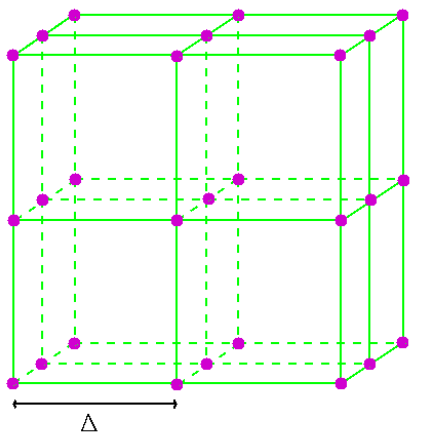
\includegraphics[scale=0.3]{img/cap02/scGrid}}
    \subfigure[\emph{body centered cubic grid (\emph{bcc})}]{\label{fig:bcc}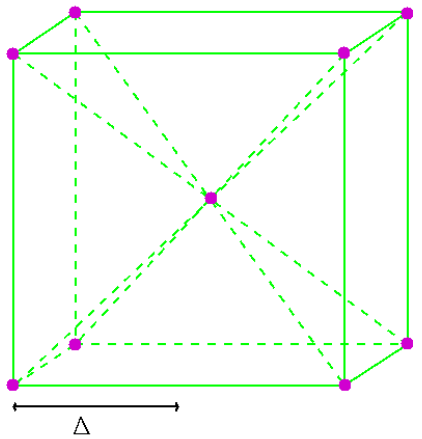
\includegraphics[scale=0.3]{img/cap02/bccGrid}}
    \subfigure[\emph{face centered cubic grid (\emph{fcc})}]{\label{fig:fcc}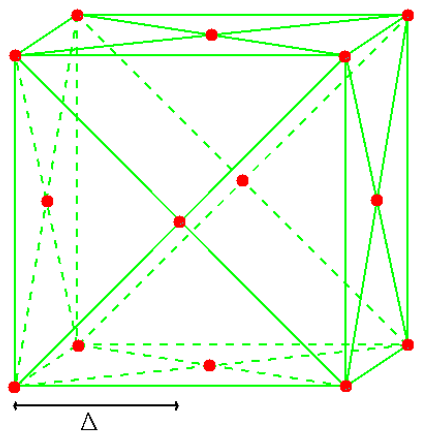
\includegraphics[scale=0.3]{img/cap02/fccGrid}}
  \end{center}
  \caption[Rejillas cúbicas]{Diferentes rejillas cúbicas.}
  \label{fig:cubicGrids}
\end{figure}

Definimos también las funciones $\shah_{G_\Delta}$, $\shah_{B_\Delta}$ y $\shah_{F_\Delta}$ generadas a partir de poner pulsos unitarios en las posiciones de la rejilla correspondiente.

En \cite{EdgarOptimization} se propone el siguiente criterio para elegir una distribución basado en el procesamiento de señales. Considerando que se desea aproximar una función constante por medio de \eqref{ec:modeloBlobby} con coeficientes $c_j = 1$, entonces el volumen puede expresarse como:

\begin{equation}
v(\textbf{x}) \approx \shah_{G} \circledast b(\textbf{x}),
 \label{ec:convMuestreo}
\end{equation}
donde el operador $\circledast$ representa la convolución y $\shah_{G}$ un tren de pulsos unitarios colocados sobre cierta rejilla $G$.
%Se ha mostrado en \cite{EdgarOptimization} que los parámetros de una función base que son ideales para hacer reconstrucción, no son necesariamente los mejores para hacer visualización. Por lo que se requiere de alguna manera de optimizar los parámetros del blob $m$, $\alpha$ y $a$ de tal manera que formen una superficie suave.

%Primeramente podemos ver de la figura \ref{fig:blobSmothnessVariation} que mientras $m$ aumenta los blobs tienen valores mas pequeños conforme se alejan del centro, es decir su tasa de caída aumenta, lo cual no es conveniente para nuestros propósitos. Además hacer los cálculos del blob mientras $m$ aumenta es cada vez mas costoso (ver ecuación \eqref{ec:blob}). Para $m = 2$ el blob tiene un comportamiento suave y dado que existen $m - 1 = 1$ derivadas nos aseguramos que el gradiente del blob existe. Por estas razones en este trabajo fijamos el parámetro $m = 2$.

%Una vez que tenemos fijo ese parámetro, quedan por determinar $\alpha$ y $a$. Siguiendo el proceso descrito en \cite{Edgar:Thesis} y en \cite{EdgarOptimization} es razonable elegir parámetros tales que una combinación lineal de blobs, con coeficientes $c_i = 1$ aproximen una función constante usando \eqref{ec:modBlobby}.

%Para saber en donde colocar los blobs es necesario definir arreglos de puntos en el espacio 3D llamados rejillas. En particular son de nuestro interés tres rejillas:

Para continuar con el análisis requerimos de definir la transformada de Fourier para una función $g(\textbf{x})$ como
\begin{equation}
  \mathscr{F} (g) = \hat{g}(\bm \xi) = \int \limits_{\mathbb{R}^n} g(\textbf{x}) e^{-i 2 \pi \left\langle \textbf{x}, \bm \xi\right\rangle } d\textbf{x},
  \label{ec:fourierTransform}
\end{equation}
donde $\left\langle \textbf{x}, \bm \xi \right\rangle$ representa el producto interno entre los vectores $\textbf{x}$ y $\bm \xi$. Se hace notar que seguimos la convención de usar $\hat{g}$ en vez de $\mathscr{F} (g)$ para denotar la transformada de Fourier de $g$. Se adopta también la convención de usar $\bm \xi$ como un vector en el espacio de Fourier y de $R = |\bm \xi|$. Además representar la transformada de Fourier de $f$ como $\hat{f}$, como se indica en \eqref{ec:fourierTransform}.

En \cite{BlobsMate} Lewitt proporciona una la siguiente forma de calcular la transformada de Fourier del blob \eqref{ec:blob} cuando $m = 2$.

\begin{equation}
\label{ec:blobFT}
 \hat{b}(2, \alpha, a; R) = \dfrac{(2 \pi)^{3/2} a^3 \alpha^2}{I_2(\alpha)}\begin{cases}
            \dfrac{ I_{ 7 / 2 } \left( \sqrt{ \alpha^{2} - (2 \pi a R)^{2}}  \right) } { \left( \sqrt{\alpha^2 - (2 \pi a R) ^2}  \right)^{ 7 / 2 }}, & \text{ si $2 \pi a R \leq \alpha$,} \\
            \dfrac{ J_{ 7 / 2 } \left( \sqrt{ (2 \pi a R)^{2} - \alpha^{2}}  \right) } { \left( \sqrt{(2 \pi a R)^{2} - \alpha^{2}}  \right)^{ 7 / 2 }}, & \text{ si $2 \pi a R \geq \alpha$,} \\
            \end{cases}
\end{equation}
en donde $J_i$ es la función Bessel de orden $i$. Existe una relación entre la convolución y la transformada de Fourier dada por el siguiente teorema
\begin{teoSN}[Convolución]
Sean $f$ y $g$ dos funciones en $\mathbb{R}^{n}$, entonces 
\begin{eqnarray}
 \label{ec:convTheorem}
 \widehat{f \circledast g} & = & \hat{f} \times \hat{g}, \\
 \nonumber
  \widehat{f \times g} & = & \hat{f} \circledast \hat{g}. 
\end{eqnarray}
\end{teoSN}
El operador $\times$ es la multiplicación punto a punto. Por lo tanto, la convolución de \eqref{ec:convMuestreo} puede expresarse en el espacio de Fourier como:

\begin{equation}
 \hat{v}(\textbf{x}) \approx \widehat{\shah} \times \hat{b} (\bm \xi).
 \label{ec:muestreoConvolucion}
\end{equation}

En \cite{Edgar:Thesis} se obtienen formulas para la transformada de Fourier de las rejillas antes expuestas, definidas como:
\begin{eqnarray}
 \label{ec:scFt}
 \widehat{\shah_{G_\Delta}} & = \frac{1}{\Delta^3} \shah_{G_{1 / \Delta}}, \\
 \label{ec:bccFt}
 \widehat{\shah_{B_\Delta}} & = \frac{1}{4 \Delta^3} \shah_{F_{1 / 2 \Delta}}, \\
 \label{ec:fccFt}
 \widehat{\shah_{F_\Delta}} & = \frac{1}{2 \Delta^3} \shah_{B_{1 / 2 \Delta}}.
\end{eqnarray}
Cabe hacer notar que las rejillas \emph{bcc} y \emph{fcc} son reciprocas en el espacio de Fourier (ver \eqref{ec:bccFt} y \eqref{ec:fccFt}).

Aunque el arreglo de pulsos mas común es aquel definido por $\shah_{G_{\Delta}}$, en \cite{petersenSampling} se ha demostrado que el muestreo mas eficiente del espacio $\mathbb{R}^3$ es con $\shah_{B_{\Delta}}$. Por esa razón en el análisis de \cite{LewitPractical} se utiliza la distribución $\shah_{B}$ para el conjunto $\{ \textbf{p}_j \}$. 

Recordemos que deseamos aproximar una función constante y que la transfromada de Fourier de dicha función es un pulso en el origen. Por esta razones los autores de \cite{EdgarOptimization} sugieren que el primer cero de \eqref{ec:blobFT} caiga exactamente en el pulso mas cercano al origen del tren de pulsos $\widehat{\shah_{B_\Delta}}$, que como sabemos de \eqref{ec:bccFt} es $\frac{1}{4 \Delta^3} \shah_{F_{1 / 2 \Delta}}$.

Revisando \eqref{ec:blobFT}, como $I_m$ nunca vale cero, debemos hacer que $J_{7 / 2}(u) = 0$, el primer valor que esto ocurre es $u = 6.987932$. Por lo que debemos hacer
\begin{equation}
 \sqrt{(2 \pi a R)^2 - \alpha^2} = u,
\label{ec:alphaEcuation}
\end{equation}
de donde sabemos que el valor para $\alpha$ debe cumplir
\begin{equation}
 \alpha = \sqrt{(2 \pi a R)^2 - u^2}.
 \label{ec:alphaEcuationSolved}
\end{equation}
%Para poder aproximar una función constante usando \eqref{ec:modBlobby} colocando los blobs en alguna de las rejillas es necesario hacer una convolución de la rejilla con el blob. Pero hacer la convolución en el espacio real es equivalente a multiplicar la transformada de Fourier del blob y de la rejilla en el espacio de Fourier, es decir

% \begin{equation}
%   v(\textbf{x}) \approx \sum \limits_{j = 1}^{J} c_j b_j (\textbf{x}) \approx \shah \circledast b(\textbf{x})
% \label{ec:funConstante}
% \end{equation}

% En el espacio real es equivalente a:
% 
% \begin{equation}
%   v(\bm \xi) \approx \widehat{b_j (\textbf{x})} \times \widehat{\shah} 
% \label{ec:funConstanteFourier}
% \end{equation}
% 
% En el espacio de Fourier. Sabemos de \cite{EdgarOptimization} que las transformadas de Fourier de las rejillas son:
% 

% 
% Para poder aproximar de manera correcta una función constante (que en el espacio de Fourier es un pulso en el origen) es necesario seleccionar un blob $b$ tal que $\widehat{b_j}$ vale cero en las posiciones de $\widehat{\shah}$ mas cercanas al origen. Dado \eqref{ec:blobFT} nos dice $\widehat{b}$ y las funciones $I_{7/2}$ nunca tienen el valor de cero debemos usar $J_{7/2}$. El valor mas pequeño de $x$ para el que $J_{7/2}(x) = 0$ toma el valor de cero es $x \approx 6.987932 = u$. Entonces debemos resolver para $\alpha$ la siguiente ecuación:
% 
La ecuación \eqref{ec:alphaEcuationSolved} permite relacionar el tamaño del blob $a$ y la separación de la rejilla $\Delta$ con la forma del blob $\alpha$. Para mas detalles de esta relación pueden verse \cite{Edgar:Thesis} y \cite{EdgarOptimization}. A pesar de que el análisis anterior produce buenos resultados para reconstrucción a partir de proyecciones, en \cite{EdgarOptimization} se demostró que produce artefactos al momento de visualizar una función $v$ aproximada por \eqref{ec:modeloBlobby}.

Para distintas rejillas el valor de $R$ en \eqref{ec:alphaEcuationSolved} es también diferente. En cada rejilla debe ser el lugar del vecino mas cercano en el espacio de Fourier. Usaremos $\lambda$ para denotar la separación de los puntos de las rejillas en el espacio de Fourier. 

Para la rejilla \emph{sc} sabemos que su transformada en el espacio de Fourier es otra rejilla \emph{sc} por \eqref{ec:scFt}. Por lo tanto sus vecino mas cercano esta a distancia $R = \lambda$, ver la Figura \ref{fig:sc}. Pero sabemos también de \eqref{ec:scFt} que en Fourier $\lambda = \frac{1}{\Delta}$, por lo tanto $R = \frac{1}{\Delta}$ y el valor de $\alpha$ es
\begin{equation}
  \alpha = \sqrt{4 \pi^2 \left( \frac{a}{\Delta} \right) ^2 - u^2}.
  \label{ec:deltaSC}
\end{equation}
 
De \eqref{ec:bccFt} se puede ver que la transformada de Fourier de \emph{bcc} es la rejilla \emph{fcc} por lo tanto estamos a distancia $R = \lambda\sqrt{2}$ ver Figura \ref{fig:fcc} pero sabemos que la separación de la rejilla transformada esta colocada a distancia $\lambda = \frac{1}{2 \Delta}$ (ver \eqref{ec:fccFt}). Por lo tanto el valor es $R = \lambda\sqrt{2} = \frac{1}{\sqrt{2} \Delta}$ y el valor de $\alpha$ es:
\begin{equation}
  \alpha = \sqrt{2 \pi^2 \left( \frac{a}{\Delta} \right) ^2 - u^2}.
  \label{ec:deltaBCC}
\end{equation}

Por último en la rejilla \emph{fcc} su transformada es la rejilla \emph{bcc} por lo tanto estamos a distancia $R = \lambda\sqrt{3}$; Figura \ref{fig:bcc}, pero la separación de la rejilla transformada esta colocada a distancia $\lambda = \frac{1}{2 \Delta}$. Por lo tanto el valor es $R = \lambda\sqrt{3} = \frac{\sqrt{3}}{2\Delta}$ y el valor de $\alpha$ es: 
\begin{equation}
  \alpha = \sqrt{3 \pi^2 \left( \frac{a}{\Delta} \right) ^2 - u^2}.
  \label{ec:deltaFCC}
\end{equation}

Tenemos ahora una relación para $\alpha$ en función de $a$ y $\Delta$ para cada rejilla. Lo único que nos resta por determinar es cual es el valor de $a$ ideal en cada caso.

Continuando con el procedimiento descrito en \cite{EdgarOptimization}, se propone el siguiente criterio. Dos blobs colocados en puntos mas cercanos de alguna rejilla, con coeficientes $c_1 = c_2 = 1$, al visualizarse con un umbral de $t = 0.5$ deben formar la primer superficie convexa.

Esto quiere decir que se ponen dos blobs iguales en puntos cercanos de la rejilla, estos blobs forman una superficie implícita como las de la Figura \ref{fig:blobSmothness}. Cuando esta superficie es umbralizada a $t = 0.5$, se busca que la figura que formen sea la primera superficie convexa. Si los blobs tienen un $a$ muy grande la superficie tiende a ser muy convexa, si por el contrario $a$ es pequeño la superficie sera cóncava. En la Figura \ref{fig:contornos} se muestran contornos de dichas superficies. En el primer caso, Figura \ref{fig:surfConcava} $a$ es pequeña y la superficie es cóncava. En el segundo caso, $a$ es grande y la superficie es muy convexa, ver la Figura \ref{fig:surfConvexa}. El último caso Figura \ref{fig:surfIdeal} muestra la superficie que estamos buscando.

\begin{figure}[htp]
  \begin{center}
    \subfigure[Superficie cóncava]{\label{fig:surfConcava}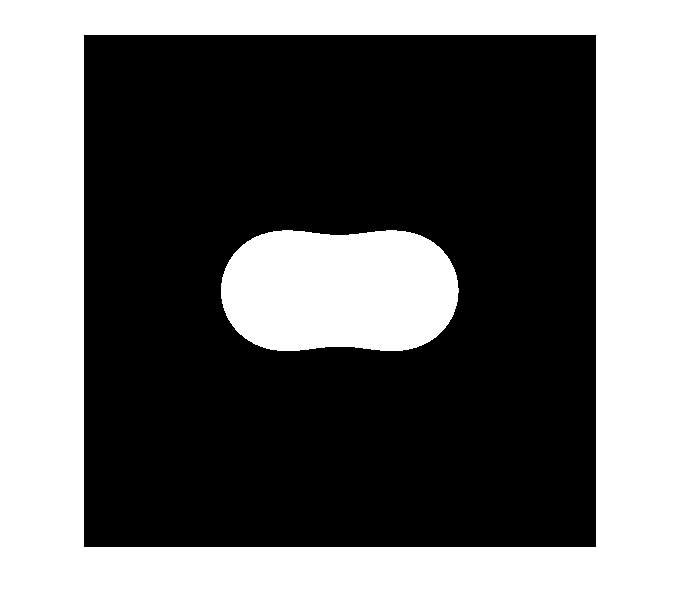
\includegraphics[scale=0.25]{img/cap02/flaco}}     
    \subfigure[Superficie demasiado convexa]{\label{fig:surfConvexa}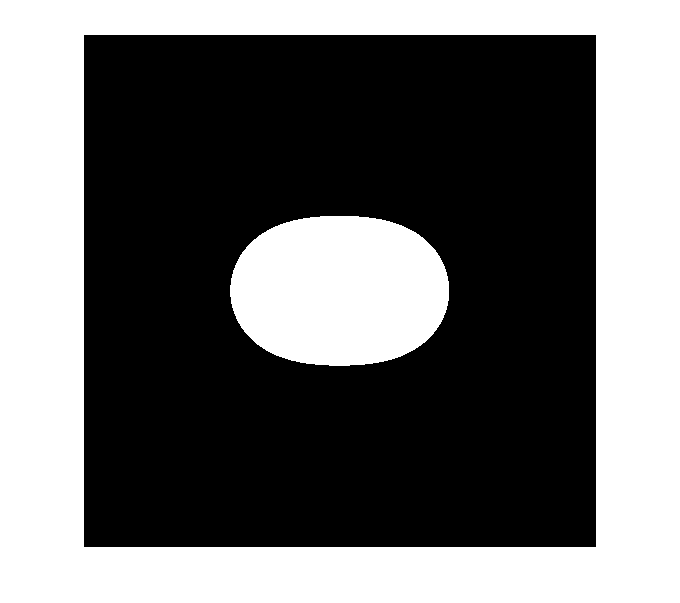
\includegraphics[scale=0.25]{img/cap02/gordo}}
    \subfigure[Primer superficie convexa]{\label{fig:surfIdeal}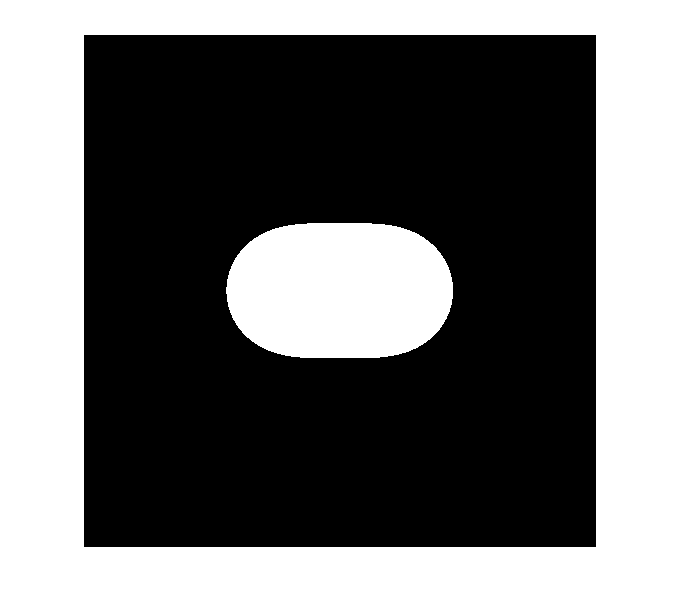
\includegraphics[scale=0.25]{img/cap02/ideal}}
  \end{center}
  \caption[Contorno de la superficie formada por dos blobs con los mismos parámetros en puntos vecinos de una rejilla y umbralizada a $t = 0.5$]{Contorno de la superficie formada por dos blobs con los mismos parámetros en puntos vecinos de una rejilla y umbralizada a $t = 0.5$.}
  \label{fig:contornos}
\end{figure}

Para obtener el blob óptimo para visualización se uso el siguiente criterio. Usamos $\Delta$ en cada rejilla tal que $R = 1$. Luego se hizo una búsqueda numérica variando el valor de $a$ y construyendo blobs que satisfagan la correspondiente ecuación \eqref{ec:alphaEcuationSolved} de su rejilla. Los resultados obtenidos se muestran en la Tabla \ref{table:resultadosBlobs}.
%Radius:  2.4000717163085934	Alpha: 13.3633110396768338
%Para bcc

%Radius:  2.4000717163085934	Alpha: 13.3633110396768320
%Para fcc

%Radius:  1.1287071228027343	Alpha:  1.2097568760112227
%Para sc
\begin{table}
\begin{center}
  \begin{tabular}{| l | l | r |}
    \hline
    Rejilla & $a$ & $\alpha$ \\ 
    \hline
    \emph{sc} & 1.13 &  1.21 \\
    \emph{bcc} & 2.4 & 13.36 \\
    \emph{fcc} & 2.4 & 13.36 \\
    \hline
  \end{tabular}
\end{center}
\caption[Resultados de optimizar $a$ y su correspondiente $\alpha$ para las diferentes rejillas]{Resultados de optimizar $a$ y su correspondiente $\alpha$ para las diferentes rejillas.}
\label{table:resultadosBlobs}
\end{table}

Es interesante notar que debido a la relación que guardan las rejillas \emph{fcc} y \emph{bcc} en el espacio de Fourier \eqref{ec:fccFt} y \eqref{ec:bccFt}, obtuvimos el mismo blob en ambos casos. También hay que aclarar que el blob esta escalado al momento de fijar $\Delta$ y dado que las relaciones de $\alpha$ dependen del cociente $\frac{a}{\Delta}$ solo es necesario multiplicar el soporte del blob $a$ para adaptarlo al $\Delta$ del conjunto de datos.

\subsection{Ponderado de normales por medio de blobs}
\label{sec:ponderadoNormalesBlobs}
Si se conociera el conjunto de coeficientes $\{ c_j \}$ y los parámetros de los blobs $b_j$ que mejor aproximan el volumen de \eqref{ec:modeloBlobby}, podríamos calcular las normales directamente en todo el campo escalar usando \eqref{ec:gradSuperficie}. 

En nuestro caso no se tiene información del campo escalar $f$ que queremos visualizar. Pero sabemos que $g$ como en \eqref{ec:modeloBlobby} se aproxima a $f$ y a su vez $v$ es una aproximación de $g$.  Se desea visualizar a $S_{\tau}$ definido en \eqref{ec:isosupeficie} pero solo tenemos la aproximación $\mathcal{A}_{\tau}$ proveniente del Algoritmo de Artzy. Por lo tanto vamos a poner $\mathcal{A}_{\tau}$ dentro de la superficie implícita $g$ y usaremos la superficie para calcular normales de iluminación de $\mathcal{A}_{\tau}$.
%Por estas dos razones se planean calcular normales de la malla $\mathcal{A}_{\tau}$ usando el gradiente $\nabla v$ definido en \eqref{ec:gradSuperficie}.

Como la salida $\mathcal{A}_{\tau}$ del Algoritmo de Artzy esta formada por una malla que esta dentro de $g$ y se conoce la posición de los vértices de la malla podríamos calcular normales para la malla $\mathcal{A}_{\tau}$ usando el gradiente $\nabla g$ definido en \eqref{ec:gradSuperficie} y estas deben ser una buena aproximación a las normales de $S_{\tau}$.

Debido a la falta de información solo podemos usar ciertos criterios para construir la aproximación de \eqref{ec:modeloBlobby}. Los criterios propuestos son los siguientes:

\begin{itemize}
  \item Vamos a poner el conjunto $\{ \textbf{p}_j \}$ en el centro de cada vóxel de la rejilla \emph{sc}.
  \item Para todos los vóxeles que el algoritmo de Artzy encontró como interiores (Es decir que tenían un valor $v(\textbf{k}) \geq \tau$), los coeficientes serán $c_j = 1$.
  \item Para todos los vóxeles que el algoritmo de Artzy encontró como exteriores ($v(\textbf{k}) < \tau$), los coeficientes serán: $c_j = 0$.
  \item Las funciones base $\{ b_j \}$ son blobs y todos tendrán el mismo conjunto de parámetros $m$, $\alpha$ y $a$ determinados por el método expuesto en la sección anterior.
\end{itemize}

Bajo las condiciones arriba propuestas tenemos una manera de calcular \eqref{ec:gradSuperficie} y por consecuencia tenemos una manera de calcular el conjunto de vectores normales $\vec{\textbf{n}}$ en cada vértice de la malla $\mathcal{A}_{\tau}$. Usando esta información y el modelo de iluminación \eqref{ec:phongModelo} esperamos tener resultados visiblemente mas agradables que los arrojados por el Algoritmo de Artzy.

Ilustrando los criterios arriba expuestos esto quiere decir que asumiremos que hay un blob en cada vóxel que esta dentro de la malla $\mathcal{A}_{\tau}$ que como se comentó en el capitulo anterior es una superficie cerrada. Con esos blobs se forma una superficie implícita a la que le podemos calcular su normal en cualquier punto y luego usamos esa normal en los vértices de la malla $A_{\tau}$. Todo esto se simboliza en la Figura \ref{fig:ejemploNS}, donde por simplicidad se muestra en solo en 2D.

\begin{figure}[htp]
  \begin{center}
    \subfigure[Malla obtenida por el Algoritmo de Artzy $\mathcal{A}_{\tau}$]{\label{fig:ejemploMalla}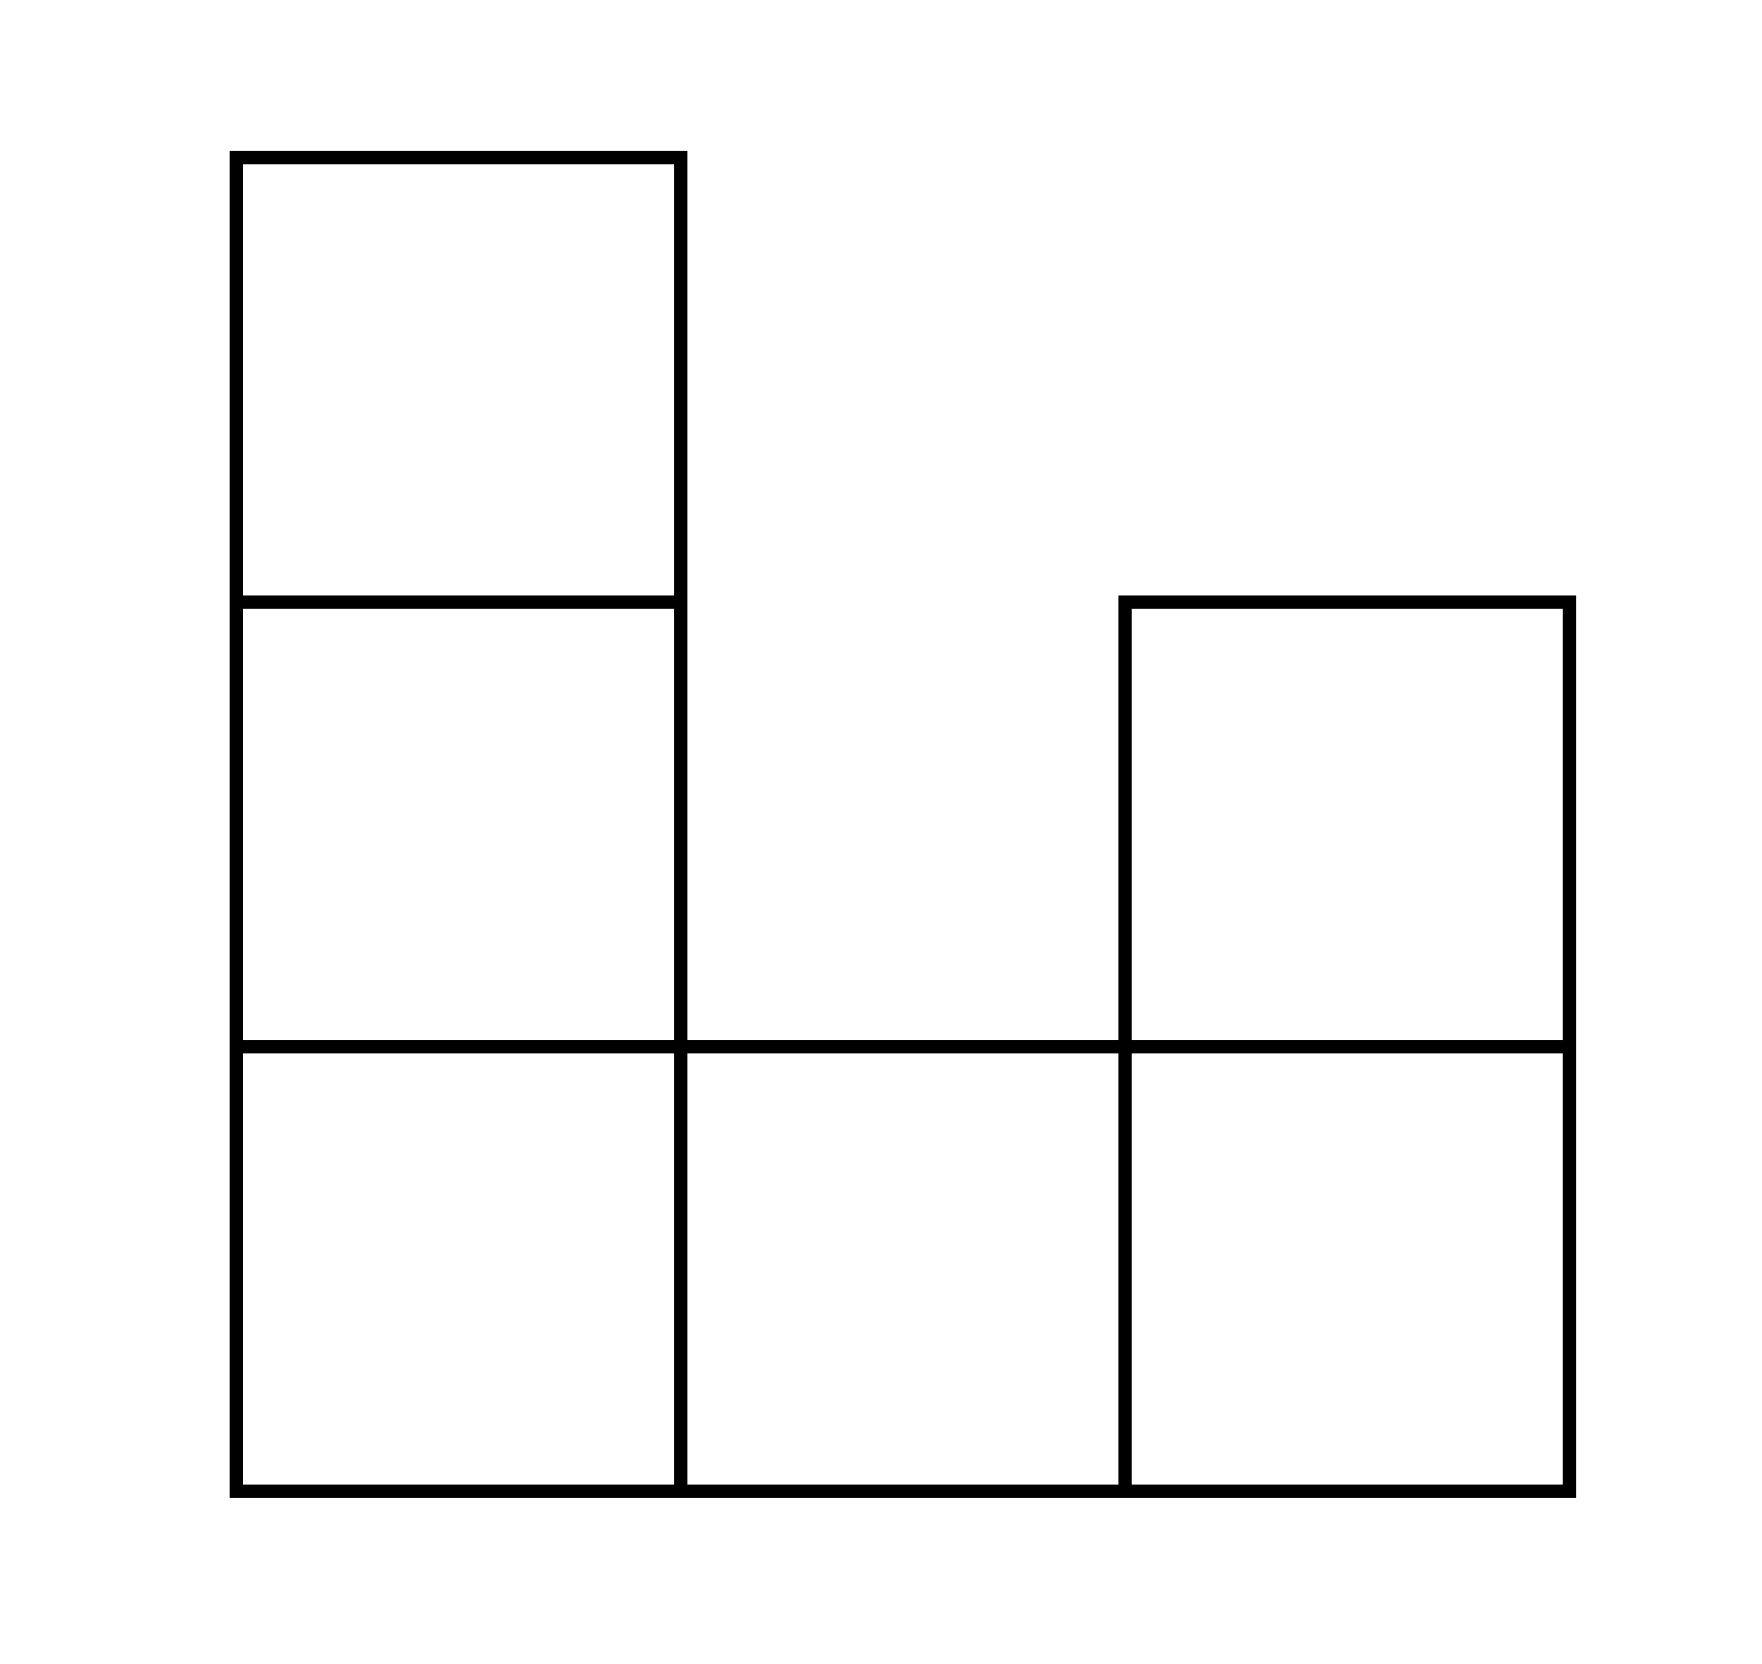
\includegraphics[scale=0.5]{img/cap02/rejillaEjemplo1}}
    \\
    \subfigure[Conjunto $\{ b_j \}$ con $c_j \neq 0$]{\label{fig:ejemploBlobs}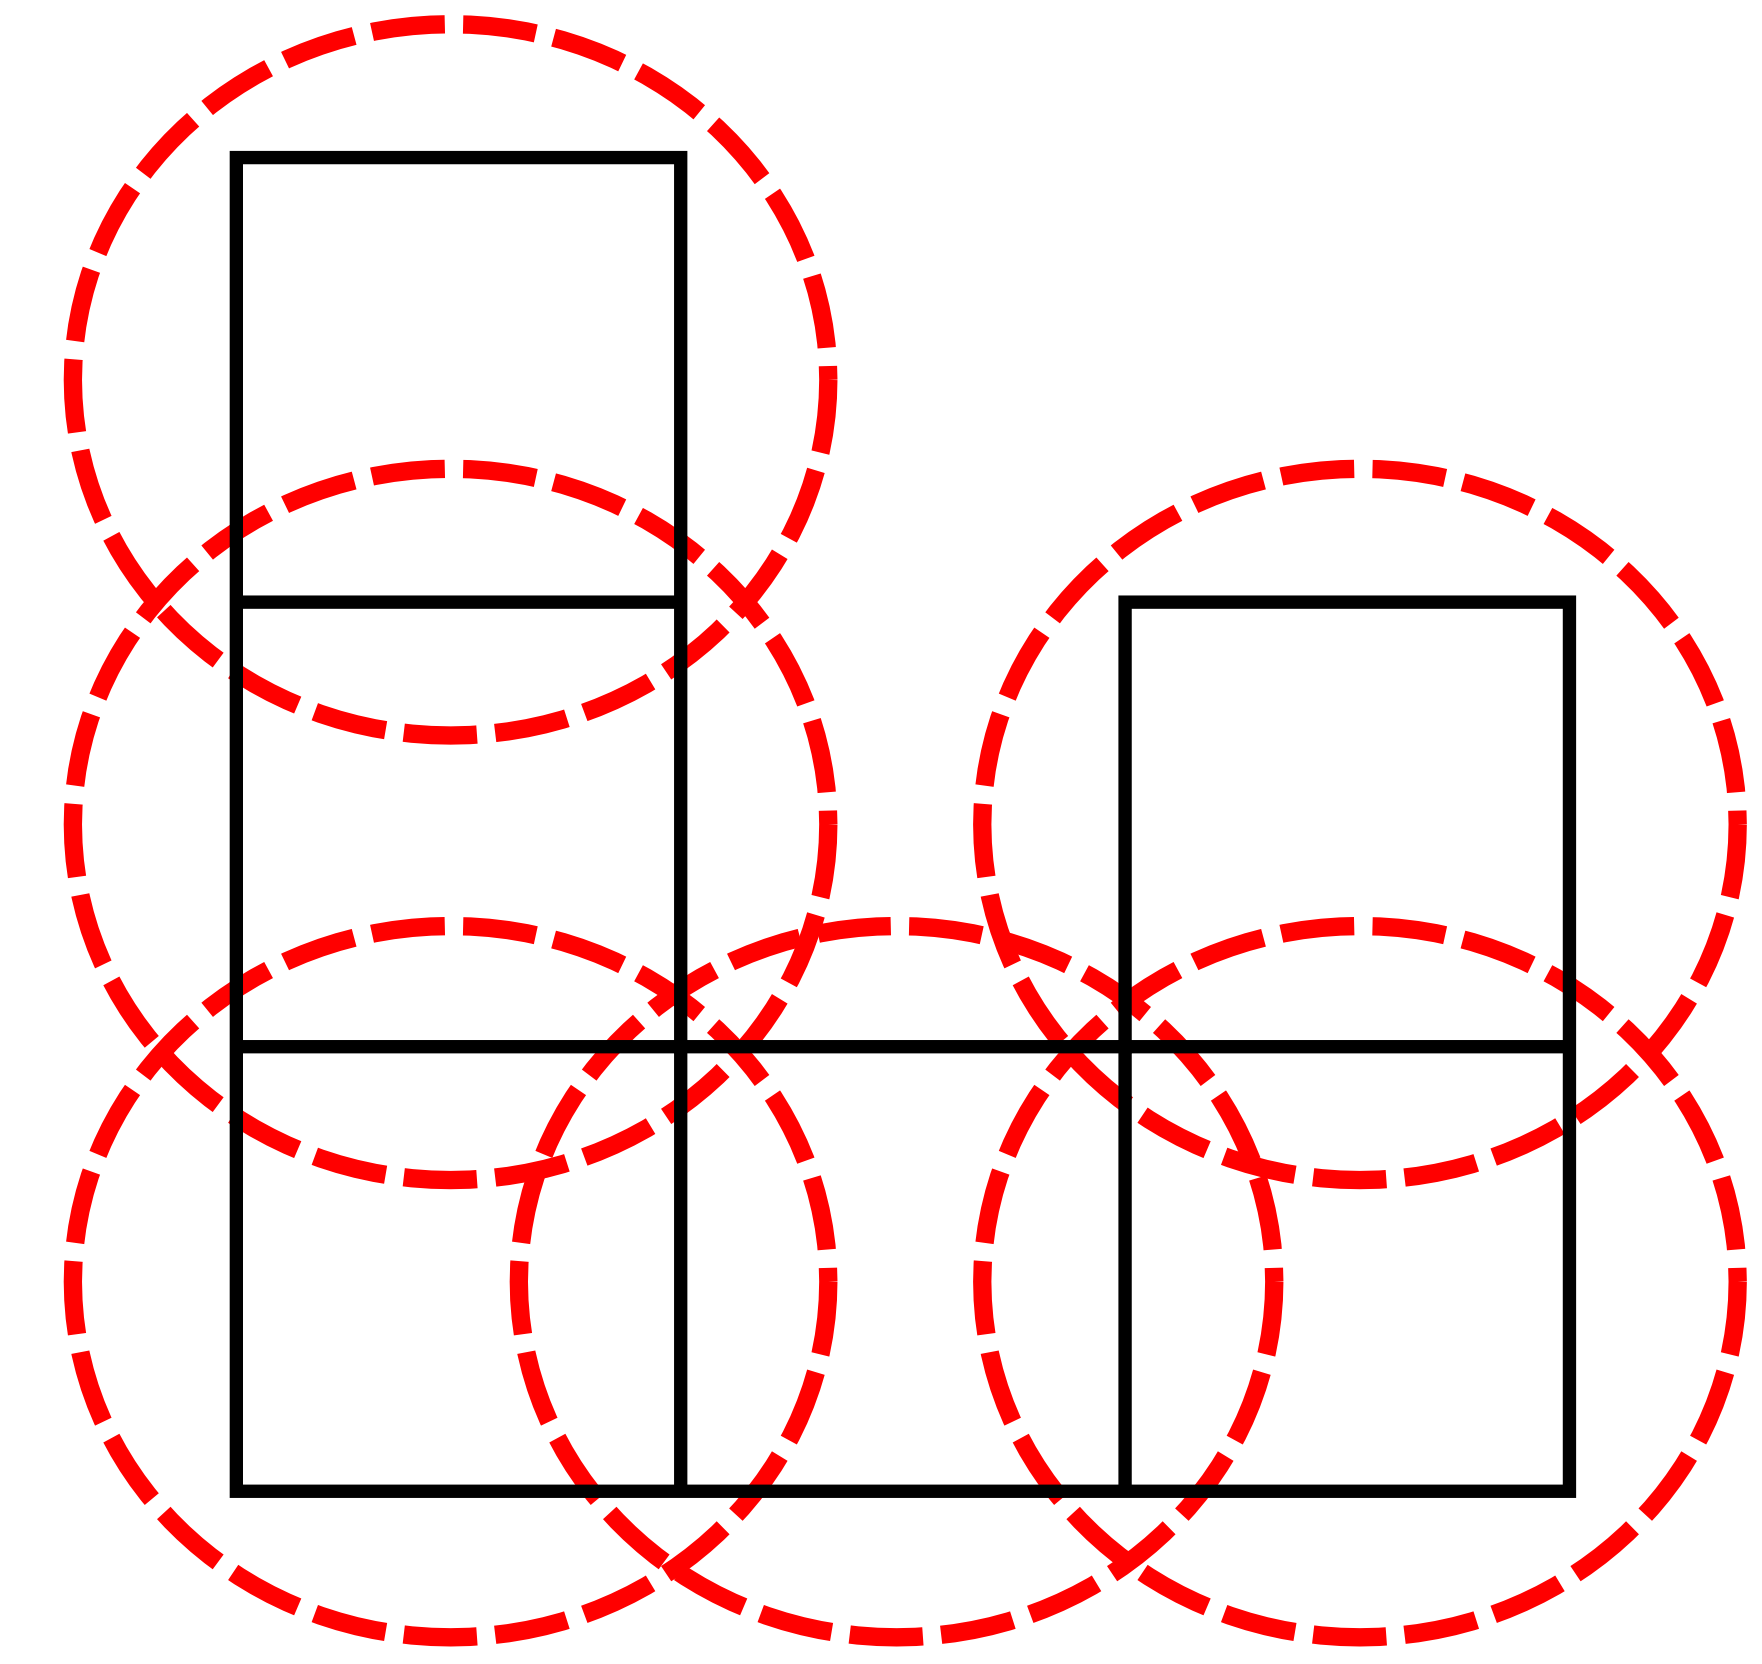
\includegraphics[scale=0.5]{img/cap02/rejillaEjemplo2}} 
    \\
    \subfigure[Superficie implicita]{\label{fig:ejemploSupImpl}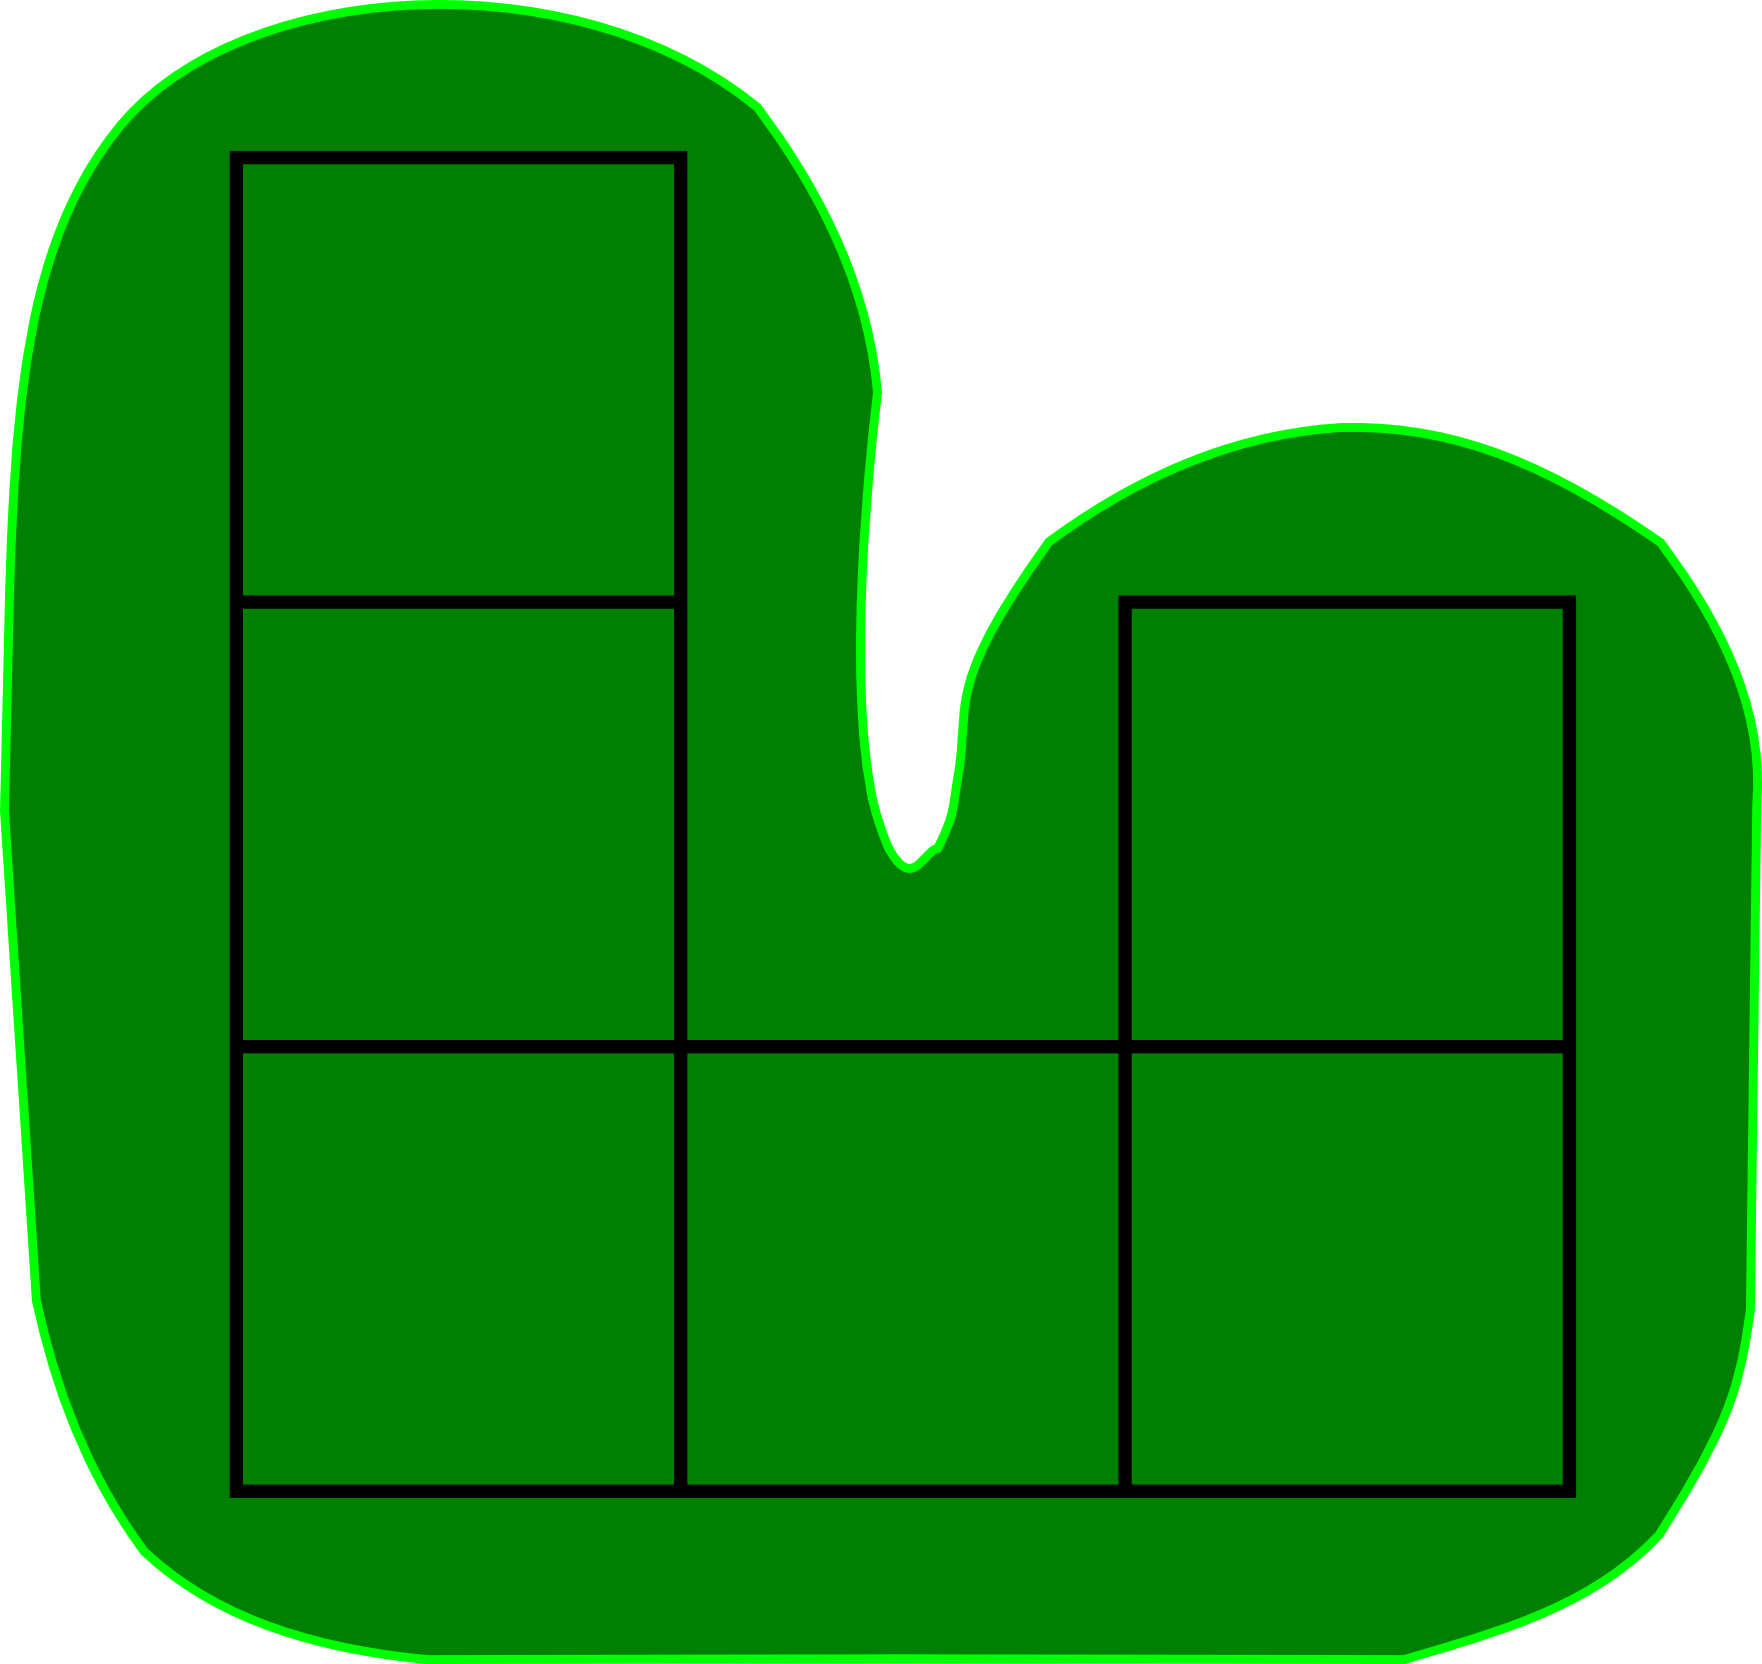
\includegraphics[scale=0.5]{img/cap02/rejillaEjemplo3}}
  \end{center}
  \caption[Ejemplo de colocación de lo blobs para visualización]{Al colocar los blobs en los centros de los vóxeles estos definen una superficie implícita en donde podemos calcular al gradiente en cada punto.}
  \label{fig:ejemploNS}
\end{figure}

En la Figura \ref{fig:ejemploMalla} se muestra una posible malla $\mathcal{A}_{\tau}$ arrojada por el Algoritmo de Artzy. Se colocan blobs $b_j$ en los centros de los vóxeles interiores de la malla $\{\textbf{p}_j\}$ estos forman una superficie implícita $g$ como la de \eqref{ec:modeloBlobby}, que se muestra en verde en la Figura \ref{fig:ejemploSupImpl}. Como $\mathcal{A}_{\tau}$ esta dentro de la superficie $g$ podemos usar \eqref{ec:gradSuperficie} para calcular el gradiente en cualquier punto $\textbf{p}$, en particular nos interesa calcularlo en los vértices de la malla $\mathcal{A}_{\tau}$.

Para hacer la ponderación de las normales de la salida del Algoritmo de Artzy, usamos el Algoritmo \ref{algo:normPond}. Las entradas de este algoritmo son la malla de salida del Algoritmo de Artzy $\mathcal{A}_{\tau}$ y los parámetros $a$, $m$ y $\alpha$ del blob usado para construir la superficie implícita.

En resumen, una vez que se tiene la aproximación $\mathcal{A}_{\tau}$, se hace el posprocesamineto descrito en el Algoritmo \ref{algo:normPond}, para obtener un conjunto de normales a la superficie, usando alguno de los blobs óptimos de la sección anterior.

\begin{algorithm}[H]
\caption{Ponderado de Normales}
\label{algo:normPond}
\begin{algorithmic}[1]
\REQUIRE Una malla de salida del algoritmo de Artzy $\mathcal{A}_{\tau}$ y los parámetros $a$, $m$ y $\alpha$ de un blob $b$.
\ENSURE Un conjunto de normales $M$ a cada punto vértice de la $\mathcal{A}_{\tau}$
\STATE Calcula el tamaño de la escena $\Gamma$ de donde viene $\mathcal{A}_{\tau}$ 
\STATE Calcula el conjunto $I$ de todos los vóxeles en $\Gamma$ interiores de la malla $\mathcal{A}_{\tau}$.
\FORALL{$\textbf{k} \in \Gamma$}
   \IF{$\textbf{k} \in I$} 
     \STATE Calcula la vecindad $N_{\textbf{k}} = \left\lbrace \textbf{a} | a > |\textbf{a} - \textbf{k}| \right\rbrace $ del punto $\textbf{k}$.     
     \FORALL{$\textbf{p} \in N_{\textbf{k}}$}
	\IF{$\textbf{p} \in \mathcal{A}_{\tau}$}
	   \STATE Calcular el vector $\textbf{q} = \textbf{p} - \textbf{k}$
	   \STATE Calcular la magnitud del gradiente $\eta = \frac{\partial}{\partial r} b (a, \alpha, m; |\textbf{q}| )$
	   \STATE Acumular a la normal $\textbf{n}_{\textbf{p}} \in M$ del punto $\textbf{p}$ la contribución de este gradiente: $\textbf{n}_{\textbf{p}} = \textbf{n}_{\textbf{p}} + \eta\frac{\textbf{q}}{|\textbf{q}|}$
	\ENDIF
     \ENDFOR
   \ENDIF
\ENDFOR
\FORALL{$\textbf{n} \in M$}
  \STATE $\textbf{n} = \frac{\textbf{n}}{|\textbf{n}|}$
\ENDFOR
\end{algorithmic}
\end{algorithm}
